% !TeX program = pdflatex
% Compile with pdfLaTeX until cross-references and the contents are stable.

\documentclass[11pt,a4paper]{article}
\usepackage[T1]{fontenc}
\usepackage[utf8]{inputenc}
\usepackage{lmodern,microtype}
% Include Unicode mappings for searchable, copyable text in the PDF.
\ifdefined\pdfgentounicode
  \input{glyphtounicode}
  \pdfgentounicode=1
\fi
\usepackage{geometry}
\geometry{left=23mm,right=23mm,top=22mm,bottom=24mm,headheight=22pt}
\usepackage{setspace}
\setstretch{1.06}
\usepackage{amsmath,amssymb,mathtools,bm}
\usepackage{array,tabularx,booktabs}
\usepackage{enumitem,xcolor,tcolorbox}
\tcbuselibrary{skins,theorems,breakable}
\usepackage{needspace,etoolbox,fancyhdr,titlesec}
\usepackage{tikz}
\usetikzlibrary{arrows.meta,calc,positioning,decorations.markings}
\usepackage[font=small,labelfont=bf]{caption}
\usepackage{hyperref}

\definecolor{ink}{HTML}{414141}
\definecolor{vuBurgundy}{HTML}{78003F}
\definecolor{blue}{HTML}{174F78}
\definecolor{navy}{HTML}{123653}
\definecolor{paleBlue}{HTML}{F1F6F9}
\definecolor{paleBurgundy}{HTML}{FAF2F6}
\definecolor{workGray}{HTML}{ABB3BB}
\definecolor{softGray}{HTML}{F5F5F5}
\color{ink}
\setlength{\parindent}{0pt}
\setlength{\parskip}{0.48em}
\setlength{\emergencystretch}{1.6em}
\raggedbottom
\clubpenalty=10000
\widowpenalty=10000
\displaywidowpenalty=10000
\setlist[enumerate]{leftmargin=1.8em,itemsep=0.25em,topsep=0.25em}
\setlist[itemize]{leftmargin=1.5em,itemsep=0.25em,topsep=0.25em}
\setcounter{tocdepth}{2}
\setcounter{secnumdepth}{2}
\numberwithin{equation}{section}
\titleformat{\section}{\Large\bfseries\color{vuBurgundy}}{\thesection}{0.65em}{}
\titleformat{\subsection}{\large\bfseries\color{blue}}{\thesubsection}{0.65em}{}
\titlespacing*{\section}{0pt}{1.5em}{0.55em}
\titlespacing*{\subsection}{0pt}{1.1em}{0.4em}
\pretocmd{\section}{\Needspace{12\baselineskip}}{}{}
\pretocmd{\subsection}{\Needspace{5\baselineskip}}{}{}
\pagestyle{fancy}
\fancyhf{}
\fancyhead[L]{\small\color{vuBurgundy}\textbf{General Relativity II}}
\fancyhead[R]{\small\color{ink!65}Lecture notes}
\fancyfoot[C]{\small\color{vuBurgundy}\thepage}
\renewcommand{\headrulewidth}{0.4pt}
\renewcommand{\headrule}{\hbox to\headwidth{\color{vuBurgundy}\leaders\hrule height\headrulewidth\hfill}\vskip-\headrulewidth}
\hypersetup{pdftitle={General Relativity II - Lecture Notes},
  pdfsubject={Metric connections, curvature, orthonormal frames, and Cartan's equations},
  colorlinks=true,linkcolor=navy,urlcolor=blue,bookmarksnumbered=true}

\newcommand{\R}{\mathbb R}
\newcommand{\dd}{\mathrm d}
\newcommand{\Cinf}{C^\infty}
\newcommand{\X}{\mathfrak X}
\newcommand{\Lie}{\mathcal L}
\newcommand{\id}{\operatorname{id}}
\newcommand{\grad}{\operatorname{grad}}
\newcommand{\GL}{\mathrm{GL}}
\newcommand{\slideref}[1]{\par\nobreak\smallskip\nobreak{\footnotesize\color{ink!60}\textsc{Source slide #1}}\par\nobreak\smallskip\nobreak}
\newcommand{\slidesref}[1]{\par\nobreak\smallskip\nobreak{\footnotesize\color{ink!60}\textsc{Source slides #1}}\par\nobreak\smallskip\nobreak}
\newcommand{\proofend}{\unskip\nobreak\hfill\(\square\)\par}
\newenvironment{proof}{\par\noindent\textit{Proof.}\ }{\proofend}

\tcbset{statement/.style={enhanced,breakable,lines before break=4,boxrule=0.65pt,arc=1.2mm,
  left=2.5mm,right=2.5mm,top=1.6mm,bottom=1.6mm,
  before skip=7pt,after skip=8pt,fonttitle=\bfseries,coltitle=white}}
\newtcbtheorem[number within=section]{definition}{Definition}{statement,unbreakable,
  title after break={Definition~\thetcbcounter\ (continued)},
  colback=paleBlue,colframe=blue,colbacktitle=blue}{def}
\newtcbtheorem[use counter from=definition]{theorem}{Theorem}{statement,
  title after break={Theorem~\thetcbcounter\ (continued)},
  colback=paleBurgundy,colframe=vuBurgundy,colbacktitle=vuBurgundy}{thm}
\newtcbtheorem[use counter from=definition]{proposition}{Proposition}{statement,
  title after break={Proposition~\thetcbcounter\ (continued)},
  colback=paleBurgundy,colframe=vuBurgundy,colbacktitle=vuBurgundy}{prop}
\newtcbtheorem[use counter from=definition]{examplebox}{Example}{statement,
  title after break={Example~\thetcbcounter\ (continued)},
  colback=softGray,colframe=ink!45,colbacktitle=ink!65}{ex}
\newtcolorbox{remarkbox}[1][Remark]{statement,title={#1},title after break={#1 (continued)},
  colback=paleBurgundy,colframe=vuBurgundy,colbacktitle=vuBurgundy}
% Blank writing space that can continue across a page break.
\newcommand{\workingspace}[1]{%
  \par
  \begingroup
  \offinterlineskip
  \dimen0=#1\relax
  \loop\ifdim\dimen0>0pt
    \dimen2=5mm
    \ifdim\dimen0<\dimen2
      \dimen2=\dimen0
    \fi
    \hbox to \linewidth{%
      \vrule width 0pt height \dimen2 depth 0pt
      \hfil
    }%
    \penalty0
    \advance\dimen0 by -\dimen2
  \repeat
  \endgroup
}

% The optional argument specifies blank space AFTER the exercise prompt.
% Keep each exercise prompt and its writing space together on one page.
\newtcolorbox{studentwork}[2][3.3cm]{%
  enhanced,
  unbreakable,
  colback=white,
  colframe=workGray,
  colbacktitle=softGray,
  coltitle=ink,
  title={Student work -- #2},
  title after break={Student work -- #2 (continued)},
  fonttitle=\bfseries,
  boxrule=0.6pt,
  arc=1mm,
  left=3mm,
  right=3mm,
  top=2mm,
  bottom=2mm,
  before skip=8pt,
  after skip=11pt,
  after upper={\workingspace{#1}}
}

\begin{document}
\hypersetup{pageanchor=false}
\begin{titlepage}
\centering
\vspace*{2.2cm}
{\Huge\bfseries\color{vuBurgundy}General Relativity II\par}
\vspace{0.45cm}
{\LARGE\color{vuBurgundy}Lecture Notes\par}
\vspace{0.8cm}
{\large Metric connections, curvature,\\[0.25em]
orthonormal frames, and Cartan's equations\par}
\vfill
{\small Curvature measures the leading change under\\[0.25em]
parallel transport around an infinitesimal loop.\par}
\end{titlepage}
\hypersetup{pageanchor=true}
\pagenumbering{roman}
{\small\setstretch{1.0}\tableofcontents}
\clearpage
\pagenumbering{arabic}

\section{The metric and covariant differentiation}
\label{gr2:sec:metric-connection}
\slideref{1}

GR1 introduced the geometric structures needed to describe fields on a
manifold. The metric pairs vectors at the same point, while a connection
defines differentiation and parallel transport. We now use the metric to
select a connection and study what happens when a vector is transported
along different paths. This leads to curvature. We will calculate it both
in coordinate bases and in local orthonormal frames.

Throughout, \(M\) is a smooth \(n\)-dimensional manifold. The notation
\(\Cinf(M)\) denotes its smooth real functions and \(\X(M)\) its smooth
vector fields. In a chart \((U,x)\), write
\(\partial_i=\partial/\partial x^i\), with \(i,j,k=1,\ldots,n\).
In general formulas, coordinate indices range over the dimension of the
chart. When specializing to spacetime, we use Greek indices
\(\mu,\nu,\rho=0,1,2,3\). Repeated upper and lower indices are summed. All fields and
coordinate changes are smooth.

\subsection{The metric and its inverse}
\slidesref{2--3}

A metric \(g\) assigns to each \(p\in M\) a symmetric, nondegenerate
bilinear form
\[
 g_p:T_pM\times T_pM\longrightarrow\R
\]
whose components depend smoothly on \(p\). Nondegeneracy means that
\(g_p(v,w)=0\) for every \(w\in T_pM\) implies \(v=0\). In coordinates,
\begin{equation}
 g=g_{ij}\,\dd x^i\otimes\dd x^j,
 \qquad g_{ij}=g(\partial_i,\partial_j),
 \qquad g(v,w)=g_{ij}v^iw^j.
 \label{gr2:eq:metric}
\end{equation}
Thus \(g_{ij}\) are the components of the metric tensor, and the matrix
\((g_{ij})\) is invertible at every point.

The signature of a nondegenerate metric is locally constant. We take it
to be fixed on the region under consideration. For a Riemannian metric,
the quadratic form is positive definite and gives ordinary lengths and
angles. For a Lorentzian spacetime metric we use signature
\((+,-,-,-)\). A nonzero vector is timelike, null, or spacelike according
as \(g(v,v)\) is positive, zero, or negative. In particular,
\(\sqrt{|g(v,v)|}\) is not a norm, since a nonzero null vector has zero
value. Euclidean angle formulas require a positive-definite metric,
such as \(-g\) on an observer's rest space.

The familiar line-element notation abbreviates the symmetric tensor
in \eqref{gr2:eq:metric},
\[
 \dd s^2=g_{ij}\,\dd x^i\dd x^j.
\]
Here \(\dd x^i\dd x^j\) denotes ordinary multiplication in the
quadratic expression. It is not the wedge product
\(\dd x^i\wedge\dd x^j\).
For a curve \(\gamma:I\to U\) in this chart, with coordinate functions
\(x^i(t)=x^i(\gamma(t))\), its meaning is
\[
 \gamma^*g
 =g_{ij}(\gamma(t))\dot x^i(t)\dot x^j(t)\,\dd t\otimes\dd t.
\]
It describes the metric along the curve. A finite coordinate difference
between two arbitrary points does not in general give their interval
through a single evaluation of \(g_{ij}\).

The inverse matrix defines the inverse metric,
\begin{equation}
 g^{ik}g_{kj}=\delta^i{}_j,
 \qquad
 g^{-1}=g^{ij}\partial_i\otimes\partial_j.
 \label{gr2:eq:inverse-metric}
\end{equation}
It pairs covectors. Raising and lowering indices expresses the inverse
maps between tangent and cotangent spaces,
\[
 v_i=g_{ij}v^j,
 \qquad \alpha^i=g^{ij}\alpha_j.
\]
These are metric-dependent operations. They are distinct from the
metric-independent pairing \(\alpha(v)=\alpha_i v^i\).

For example, Euclidean space has \(g_{ij}=\delta_{ij}\) in Cartesian
coordinates, while Minkowski spacetime has
\(g_{\mu\nu}=\eta_{\mu\nu}=\operatorname{diag}(1,-1,-1,-1)\)
in inertial coordinates with \(x^0=ct\). The sphere of radius \(a>0\)
has
\[
 \dd s^2=a^2\dd\vartheta^2+a^2\sin^2\vartheta\,\dd\varphi^2
\]
on an angular chart with \(0<\vartheta<\pi\) and a chosen open longitude
interval. The component matrices differ because both geometry and
choice of coordinates enter their description. Curvature will separate
these two effects.

\begin{studentwork}[2.6cm]{differentiating the inverse metric}
Differentiate \(g^{ik}g_{kj}=\delta^i{}_j\) to show that
\(\partial_\ell g^{ij}=-g^{im}g^{jn}\partial_\ell g_{mn}\).
\end{studentwork}

\subsection{A connection and its action on tensors}
\slidesref{4--6}

Coordinate differentiation of vector components alone does not give a
vector. Under a position-dependent change of coordinates, differentiating
the component transformation also differentiates the Jacobian. The
connection terms compensate for this extra contribution.

An affine connection is a real-bilinear map
\(\nabla:\X(M)\times\X(M)\to\X(M)\) satisfying
\begin{equation}
 \nabla_{fX}Y=f\nabla_XY,
 \qquad
 \nabla_X(fY)=X(f)Y+f\nabla_XY,
 \qquad f\in\Cinf(M).
 \label{gr2:eq:connection-axioms}
\end{equation}
Linearity over smooth functions in the first argument means that the
direction at a point is sufficient. The second argument must be a field
near that point because it is being differentiated. Define
\[
 \nabla_{\partial_i}\partial_j=\Gamma^k{}_{ij}\partial_k.
\]
The first lower index of \(\Gamma^k{}_{ij}\) specifies the direction of
differentiation. Expanding \(Y=Y^j\partial_j\) using
\eqref{gr2:eq:connection-axioms} gives
\begin{equation}
 \nabla_XY=X^i(\nabla_iY)^k\partial_k,
 \qquad
 (\nabla_iY)^k=\partial_iY^k+\Gamma^k{}_{ij}Y^j.
 \label{gr2:eq:vector-derivative}
\end{equation}
We also use the conventional component notation \(\nabla_iY^k\) for
\((\nabla_iY)^k\). It includes the connection term and does not mean
ordinary differentiation of the scalar component function \(Y^k\).

The connection extends to tensor fields by setting \(\nabla_Xf=X(f)\),
using the tensor product rule, and requiring differentiation to commute
with contractions. For a one-form \(\alpha\), the last requirement gives
\[
 X\bigl(\alpha(Y)\bigr)
 =(\nabla_X\alpha)(Y)+\alpha(\nabla_XY).
\]
Taking \(X=\partial_i\) and \(Y=\partial_j\) gives
\[
 \partial_i\alpha_j
 =(\nabla_{\partial_i}\alpha)(\partial_j)
   +\alpha(\Gamma^k{}_{ij}\partial_k)
 =\nabla_i\alpha_j+\Gamma^k{}_{ij}\alpha_k.
\]
Rearranging determines
\begin{equation}
 \nabla_i\alpha_j=\partial_i\alpha_j-\Gamma^k{}_{ij}\alpha_k.
 \label{gr2:eq:covector-derivative}
\end{equation}
The minus sign makes the two connection contributions cancel when a
vector and a covector are contracted.

Each upper index contributes a positive connection term, and each lower
index a negative one. For a tensor of type \((r,s)\), this gives
\begin{equation}
 \begin{aligned}
 \nabla_k T^{i_1\cdots i_r}{}_{j_1\cdots j_s}
 ={}&\partial_k T^{i_1\cdots i_r}{}_{j_1\cdots j_s}\\
 &+\sum_{a=1}^{r}\Gamma^{i_a}{}_{k\ell}
    T^{i_1\cdots \ell\cdots i_r}{}_{j_1\cdots j_s}\\
 &-\sum_{b=1}^{s}\Gamma^\ell{}_{k j_b}
    T^{i_1\cdots i_r}{}_{j_1\cdots \ell\cdots j_s}.
 \end{aligned}
 \label{gr2:eq:tensor-derivative}
\end{equation}
Here \(a\) and \(b\) only count index slots. In each summand, \(\ell\)
occupies the indicated slot. For fixed \(X\), \(\nabla_XT\) has the same
tensor type as \(T\). Retaining the direction as an extra covariant
argument gives \(\nabla T\), a tensor of type \((r,s+1)\).

The coefficients \(\Gamma^k{}_{ij}\) themselves are not tensor components.
For overlapping coordinates \(x^i\) and \(x^{i'}\), they obey
\begin{equation}
 \Gamma^{k'}{}_{i'j'}
 =\frac{\partial x^{k'}}{\partial x^k}
  \frac{\partial x^i}{\partial x^{i'}}
  \frac{\partial x^j}{\partial x^{j'}}\Gamma^k{}_{ij}
 +\frac{\partial x^{k'}}{\partial x^k}
  \frac{\partial^2x^k}{\partial x^{i'}\partial x^{j'}}.
 \label{gr2:eq:connection-transformation}
\end{equation}
This follows by differentiating
\(\partial_{j'}=(\partial x^j/\partial x^{j'})\partial_j\)
with \(\nabla_{\partial_{i'}}\). The second derivative is precisely the
term absent from a tensor transformation law. Nonzero connection
coefficients can therefore occur in flat space.

\subsection{Metric compatibility and torsion}
\slidesref{5--7}

To make differentiation respect the metric pairing, require
\begin{equation}
 (\nabla_Xg)(Y,Z)
 =X\bigl(g(Y,Z)\bigr)
  -g(\nabla_XY,Z)-g(Y,\nabla_XZ)=0.
 \label{gr2:eq:metric-compatibility}
\end{equation}
This condition is \emph{metric compatibility}, written \(\nabla g=0\).
It does not require the scalar function \(g(Y,Z)\) to be constant for
arbitrary fields. Its change is accounted for by the changes in the two
fields. In coordinates,
\begin{equation}
 0=\nabla_i g_{jk}
 =\partial_i g_{jk}-\Gamma^\ell{}_{ij}g_{\ell k}
                         -\Gamma^\ell{}_{ik}g_{j\ell}.
 \label{gr2:eq:compatibility-components}
\end{equation}
Since covariant differentiation commutes with contraction,
\(\nabla_i\delta^j{}_k=0\). Differentiating
\eqref{gr2:eq:inverse-metric} gives
\[
 0=\nabla_i(g^{j\ell}g_{\ell k})
  =(\nabla_i g^{j\ell})g_{\ell k}
    +g^{j\ell}\nabla_i g_{\ell k}
  =(\nabla_i g^{j\ell})g_{\ell k}.
\]
Multiplying by \(g^{km}\) yields \(\nabla_i g^{jm}=0\).
Raising and lowering indices therefore commute with a metric-compatible
covariant derivative.

The \emph{torsion} of a connection is the tensor
\begin{equation}
 T(X,Y)=\nabla_XY-\nabla_YX-[X,Y].
 \label{gr2:eq:torsion}
\end{equation}
The derivatives of multiplying functions cancel, so this expression is
\(\Cinf(M)\)-linear in both arguments. Coordinate fields commute, hence
\[
 T(\partial_i,\partial_j)=T^k{}_{ij}\partial_k,
 \qquad T^k{}_{ij}=\Gamma^k{}_{ij}-\Gamma^k{}_{ji}.
\]
Thus zero torsion is equivalent to symmetry of the lower connection
indices in a coordinate basis. In a general frame, the bracket term in
\eqref{gr2:eq:torsion} must be retained.

\subsection{The Levi--Civita connection}
\slideref{7}

\begin{theorem}{The metric determines a torsion-free connection}{gr2:levi-civita}
Every smooth pseudo-Riemannian metric \(g\) determines a unique
metric-compatible, torsion-free connection. Its coordinate coefficients
are
\begin{equation}
 \Gamma^k{}_{ij}
 =\frac12g^{k\ell}
  \bigl(\partial_i g_{j\ell}+\partial_j g_{i\ell}
                         -\partial_\ell g_{ij}\bigr).
 \label{gr2:eq:christoffel}
\end{equation}
This is the \emph{Levi--Civita connection}, and its coefficients are
the \emph{Christoffel symbols} in the chosen coordinates.
\end{theorem}

To obtain the formula, write metric compatibility in three orders,
\begin{align*}
 \partial_i g_{j\ell}
 &=\Gamma^m{}_{ij}g_{m\ell}+\Gamma^m{}_{i\ell}g_{jm},\\
 \partial_j g_{i\ell}
 &=\Gamma^m{}_{ji}g_{m\ell}+\Gamma^m{}_{j\ell}g_{im},\\
 \partial_\ell g_{ij}
 &=\Gamma^m{}_{\ell i}g_{mj}+\Gamma^m{}_{\ell j}g_{im}.
\end{align*}
Add the first two equations and subtract the third. The symmetry
\(\Gamma^m{}_{ij}=\Gamma^m{}_{ji}\) cancels four terms and combines the
remaining two,
\[
 \partial_i g_{j\ell}+\partial_j g_{i\ell}-\partial_\ell g_{ij}
 =2g_{m\ell}\Gamma^m{}_{ij}.
\]
Multiplication by \(g^{k\ell}/2\) gives
\eqref{gr2:eq:christoffel}. Any connection with the required properties
must have these coefficients, proving uniqueness.

For existence, define a connection on each coordinate domain using
\eqref{gr2:eq:christoffel} and \eqref{gr2:eq:vector-derivative}. Its
coefficients are smooth and symmetric in \(i,j\). Substitution in
\eqref{gr2:eq:compatibility-components} verifies metric compatibility.
On overlapping domains the two local connections have the same required
properties, so uniqueness makes them agree. They consequently define a
connection on all of \(M\). This is the coordinate construction of the
connection treated intrinsically in GR1.

\paragraph{Coordinates adapted to one point.}
\label{gr2:normal-point}
The coordinate construction in GR1 can now be summarized directly.
Start with coordinates centered at \(p\), and define new coordinates
\(y^i\) near \(p\) by
\[
 x^i=y^i-\frac12\Gamma^i{}_{jk}(p)y^jy^k.
\]
The Jacobian at \(p\) is the identity, so this is locally invertible.
The second derivatives at \(p\) are
\[
 \left.\frac{\partial^2x^i}{\partial y^j\partial y^k}\right|_p
 =-\frac12\bigl(\Gamma^i{}_{jk}(p)+\Gamma^i{}_{kj}(p)\bigr)
 =-\Gamma^i{}_{jk}(p),
\]
where the final equality uses zero torsion. Substitution into
\eqref{gr2:eq:connection-transformation} gives
\(\Gamma^{i'}{}_{j'k'}(p)=\Gamma^i{}_{jk}(p)-\Gamma^i{}_{jk}(p)=0\),
with old and new index labels identified by the identity Jacobian. For the
Levi--Civita connection, metric compatibility then gives
\(\partial_{i'}g_{j'k'}(p)=0\). A preceding linear change of coordinates
can also put \(g(p)\) into its standard diagonal form. These conditions
hold at the chosen point. They impose no vanishing condition on
derivatives of \(\Gamma\) there, and do not make the coefficients vanish
on a neighborhood.

\begin{studentwork}[2.8cm]{a conformally Euclidean metric}
For \(g_{ij}=e^{2f}\delta_{ij}\) on an open subset of \(\R^n\), derive
\[
 \Gamma^k{}_{ij}
 =\delta^k{}_j\partial_i f+\delta^k{}_i\partial_j f
  -\delta_{ij}\delta^{k\ell}\partial_\ell f.
\]
\end{studentwork}

From now on, unless stated otherwise, \(\nabla\) is the Levi--Civita
connection. The metric has supplied a definite transport rule. The next
question is whether transporting the same vector between two nearby
points gives the same result along different paths. Curvature measures
the local failure of this independence.

\section{Parallel transport and curvature}
\label{gr2:sec-curvature}
\slideref{8}

A connection specifies parallel transport along a chosen curve. It does
not generally make the result independent of the curve. In GR1, transport
around a latitude on the sphere returned a vector with a different
direction. We now examine this effect around an arbitrarily small loop.
The leading change defines curvature locally, without referring to an
embedding of the manifold in a larger space.

\subsection{Comparing two paths}

Let \(p\) lie in a coordinate chart and choose two coordinate directions
\(X=\partial_\mu\) and \(Y=\partial_\nu\), with \(\mu\ne\nu\). Keep all
other coordinates fixed. Starting at \(p\), increasing these two
coordinates by small amounts \(s\) and \(t\) produces a coordinate
rectangle. The two orders of travel reach the same point \(q\) because
coordinate vector fields commute.

\begin{center}
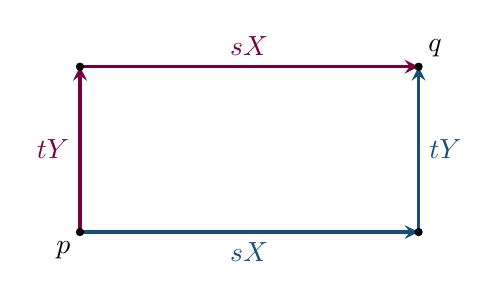
\begin{tikzpicture}[x=1cm,y=1cm,>=stealth]
\coordinate (P) at (0,0);
\coordinate (A) at (4.3,0);
\coordinate (Q) at (4.3,2.1);
\coordinate (B) at (0,2.1);
\draw[->,very thick,blue] (P) -- node[below] {\(sX\)} (A);
\draw[->,very thick,blue] (A) -- node[right] {\(tY\)} (Q);
\draw[->,very thick,vuBurgundy] (P) -- node[left] {\(tY\)} (B);
\draw[->,very thick,vuBurgundy] (B) -- node[above] {\(sX\)} (Q);
\fill (P) circle (1.5pt) node[below left] {\(p\)};
\fill (A) circle (1.5pt);
\fill (Q) circle (1.5pt) node[above right] {\(q\)};
\fill (B) circle (1.5pt);
\end{tikzpicture}
\end{center}

Write \(P_{XY}:T_pM\to T_qM\) for transport first along \(X\), then
along \(Y\), and \(P_{YX}\) for the other route. Given \(v\in T_pM\),
the vectors \(P_{XY}v\) and \(P_{YX}v\) belong to the same tangent space
and can be compared. We can also return the first vector to \(p\) along
the reverse of the second route. The resulting endomorphism
\[
 H_{s,t}=P_{YX}^{-1}P_{XY}:T_pM\longrightarrow T_pM
\]
is the transport map around the oriented loop
\(+X,+Y,-X,-Y\). A transport map around a closed loop is called a
\emph{holonomy map}.

These paths are coordinate segments. They need not be geodesics, and
\(X\) and \(Y\) need not be parallel along them. Using coordinate
segments separates the issue of comparing transport from the additional
problem of constructing curves with prescribed covariant acceleration.

\subsection{The curvature operator}
\slideref{9}

Successive covariant derivatives provide the local version of this
comparison. For general vector fields, the directions themselves need not
commute. Their failure to commute must be removed to obtain an expression
that depends only on the vectors at the point.

\begin{definition}{Curvature}{gr2:curvature}
The curvature of a connection \(\nabla\) is the operator
\begin{equation}
 R(X,Y)Z
 =\nabla_X\nabla_YZ-\nabla_Y\nabla_XZ-\nabla_{[X,Y]}Z,
 \qquad X,Y,Z\in\X(M).
 \label{gr2:eq-curvature-definition}
\end{equation}
Our component convention is
\begin{equation}
 R(\partial_\mu,\partial_\nu)\partial_\sigma
 =R^\rho{}_{\sigma\mu\nu}\partial_\rho.
 \label{gr2:eq-curvature-components}
\end{equation}
\end{definition}

The final two component indices specify the two differentiation
directions. The second index specifies the vector on which the curvature
operator acts. In particular,
\[
 R(X,Y)Z
 =R^\rho{}_{\sigma\mu\nu}Z^\sigma X^\mu Y^\nu\partial_\rho.
\]
Although its definition uses derivatives, curvature is linear over
\(\Cinf(M)\) in all three arguments. To see the cancellation in the
first argument, use
\([fX,Y]=f[X,Y]-Y(f)X\). Then
\begin{align*}
 R(fX,Y)Z
 &=f\nabla_X\nabla_YZ-Y(f)\nabla_XZ-f\nabla_Y\nabla_XZ\\
 &\quad-f\nabla_{[X,Y]}Z+Y(f)\nabla_XZ\\
 &=fR(X,Y)Z.
\end{align*}
Skew symmetry in \(X,Y\) gives the same property in the second argument.
Expanding the third argument by the product rule gives
\[
 R(X,Y)(fZ)
 =fR(X,Y)Z+
 \bigl(X(Y(f))-Y(X(f))-[X,Y](f)\bigr)Z.
\]
The last coefficient vanishes by the definition of the Lie bracket.
Thus \(R\) is a tensor field of type \((1,3)\). At a point \(p\),
\(R(X,Y)Z\) depends only on \(X_p,Y_p,Z_p\), rather than their chosen
extensions away from \(p\).

\begin{studentwork}[2.5cm]{curvature as an endomorphism}
For fixed \(u,v\in T_pM\), show that \(R_p(u,v)\) is a linear map
\(T_pM\to T_pM\). Verify \(R_p(u,v)=-R_p(v,u)\).
\end{studentwork}

\subsection{The coordinate formula}

For this calculation write \(D_\mu=\nabla_{\partial_\mu}\) as an operator
on vector fields. The connection coefficients satisfy
\[
 (D_\mu V)^\rho
 =\partial_\mu V^\rho+\Gamma^\rho{}_{\mu\sigma}V^\sigma.
\]
Apply this rule once more, keeping the direction \(\partial_\nu\)
fixed in the operator \(D_\nu\). It gives
\begin{align*}
 (D_\mu D_\nu V)^\rho
 &=\partial_\mu\partial_\nu V^\rho
   +(\partial_\mu\Gamma^\rho{}_{\nu\sigma})V^\sigma
   +\Gamma^\rho{}_{\nu\sigma}\partial_\mu V^\sigma\\
 &\quad+\Gamma^\rho{}_{\mu\lambda}\partial_\nu V^\lambda
   +\Gamma^\rho{}_{\mu\lambda}
      \Gamma^\lambda{}_{\nu\sigma}V^\sigma.
\end{align*}
Subtract the expression with \(\mu\) and \(\nu\) exchanged. The second
partial derivatives cancel. The first derivatives of \(V\) cancel in
pairs after relabelling dummy indices. Since
\([\partial_\mu,\partial_\nu]=0\), the remaining coefficient is
\begin{equation}
 \boxed{
 \begin{aligned}
 R^\rho{}_{\sigma\mu\nu}
 &=\partial_\mu\Gamma^\rho{}_{\nu\sigma}
   -\partial_\nu\Gamma^\rho{}_{\mu\sigma}\\
 &\quad+\Gamma^\rho{}_{\mu\lambda}\Gamma^\lambda{}_{\nu\sigma}
   -\Gamma^\rho{}_{\nu\lambda}\Gamma^\lambda{}_{\mu\sigma}.
 \end{aligned}}
 \label{gr2:eq-riemann-coordinate}
\end{equation}
The derivatives and products of connection coefficients combine into a
tensor even though the individual connection coefficients do not.

There are two related second derivatives in this calculation. The
iterated operator \(D_\mu D_\nu V\) differentiates a vector field with a
fixed coordinate direction in its inner operator. The full covariant
second derivative differentiates the vector-valued one-form \(\nabla V\).
Its direction index is a covariant index, so the tensor differentiation
rule contributes an additional negative connection term. Intrinsically,
\[
 (\nabla^2V)(X,Y)
 =\nabla_X\nabla_YV-\nabla_{\nabla_XY}V.
\]
Its components therefore contain an additional term,
\[
 (\nabla^2V)^\rho{}_{\mu\nu}
 =(D_\mu D_\nu V)^\rho
  -\Gamma^\lambda{}_{\mu\nu}(D_\lambda V)^\rho.
\]
Antisymmetrizing therefore gives, for a general connection,
\[
 (\nabla^2V)^\rho{}_{\mu\nu}
 -(\nabla^2V)^\rho{}_{\nu\mu}
 =R^\rho{}_{\sigma\mu\nu}V^\sigma
  -T^\lambda{}_{\mu\nu}(D_\lambda V)^\rho.
\]
The fixed-direction operator commutator has no torsion term.
For the Levi--Civita connection, \(T=0\), so both antisymmetrizations give
\begin{equation}
 (\nabla^2V)^\rho{}_{\mu\nu}
 -(\nabla^2V)^\rho{}_{\nu\mu}
 =R^\rho{}_{\sigma\mu\nu}V^\sigma.
 \label{gr2:eq-curvature-commutator}
\end{equation}
This is the meaning of the usual commutator formula when its successive
covariant derivatives are written in component notation.

\subsection{Curvature and a small loop}

The two routes agree whenever either side length vanishes. Their
difference therefore has no term depending only on \(s\) or only on
\(t\). We will calculate the first possible nonzero term, proportional
to \(st\), and then transport the difference back to \(T_pM\).

Introduce the matrices \((\Gamma_\mu)^\rho{}_{\sigma}
=\Gamma^\rho{}_{\mu\sigma}\), with \(\mu\) fixed. Along a short segment
in the \(\mu\) direction, the parallel-transport equation gives
\[
 V(s)=\bigl(I-s\Gamma_\mu(p)\bigr)V(0)+O(s^2),
\]
where \(I\) is the identity matrix in the coordinate frame. For the
second segment we must also expand the connection at its shifted
starting point. If \(p_s\) is the endpoint of the first segment, then
\[
 \Gamma_\nu(p_s)
 =\Gamma_\nu(p)+s\partial_\mu\Gamma_\nu(p)+O(s^2).
\]
The first-order segment matrices are therefore multiplied in the order
\[
 \bigl[I-t(\Gamma_\nu+s\partial_\mu\Gamma_\nu)\bigr]
 \bigl[I-s\Gamma_\mu\bigr].
\]
The right factor acts first. The product contributes
\(st\Gamma_\nu\Gamma_\mu\), while the shifted connection contributes
\(-st\partial_\mu\Gamma_\nu\). All matrices and derivatives in the
following expansion are evaluated at \(p\). Along the \(\mu\) segment,
differentiating \(V'=-\Gamma_\mu V\) once more gives
\[
 V''=-(\partial_\mu\Gamma_\mu)V-\Gamma_\mu V'
     =(\Gamma_\mu^2-\partial_\mu\Gamma_\mu)V.
\]
This determines the pure quadratic terms in the Taylor expansion.
Representing transport in the coordinate bases at the endpoints gives
\begin{align*}
 P_{XY}
 &=I-s\Gamma_\mu-t\Gamma_\nu
   +\frac{s^2}{2}(\Gamma_\mu^2-\partial_\mu\Gamma_\mu)
   +\frac{t^2}{2}(\Gamma_\nu^2-\partial_\nu\Gamma_\nu)\\
 &\quad+st(\Gamma_\nu\Gamma_\mu-\partial_\mu\Gamma_\nu)
   +O\bigl((|s|+|t|)^3\bigr).
\end{align*}
Exchanging the order of the segments leaves the pure terms unchanged
and replaces the mixed coefficient by
\(\Gamma_\mu\Gamma_\nu-\partial_\nu\Gamma_\mu\). Thus
\begin{align*}
 P_{XY}-P_{YX}
 &=-st\bigl(\partial_\mu\Gamma_\nu-\partial_\nu\Gamma_\mu
            +\Gamma_\mu\Gamma_\nu-\Gamma_\nu\Gamma_\mu\bigr)\\
 &\quad+O\bigl(|st|(|s|+|t|)\bigr).
\end{align*}
The remainder contains both side lengths because the exact difference
vanishes whenever \(s=0\) or \(t=0\). The matrix in parentheses is the
curvature matrix in \eqref{gr2:eq-riemann-coordinate}.
Finally,
\[
 H_{s,t}-I=P_{YX}^{-1}(P_{XY}-P_{YX}),\qquad
 P_{YX}^{-1}=I+O(|s|+|t|).
\]
Multiplying by the return map therefore changes only the remainder.
Returning to the starting tangent space gives
\begin{equation}
 H_{s,t}v-v
 =-st\,R_p(X_p,Y_p)v
  +O\bigl(|st|(|s|+|t|)\bigr).
 \label{gr2:eq-small-loop}
\end{equation}
The remainder is measured in any fixed norm on the finite-dimensional
space \(T_pM\). The expansion concerns fixed coordinate directions as
\(s,t\to0\).

The minus sign follows from the traversal \(+X,+Y,-X,-Y\) and
definition~\eqref{gr2:eq-curvature-definition}. Reversing the loop
reverses its leading change. The factor \(st\) is oriented coordinate
area. For a Riemannian metric, the leading physical area magnitude is
\[
 |st|\sqrt{g_p(X_p,X_p)g_p(Y_p,Y_p)-g_p(X_p,Y_p)^2}.
\]
This conversion uses the metric on the two-plane spanned by the sides.

\subsection{Coordinates and local flatness}

The normal-coordinate construction in GR1 sets the Levi--Civita
coefficients to zero at any chosen point \(p\). In such coordinates,
\eqref{gr2:eq-riemann-coordinate} becomes
\[
 R^\rho{}_{\sigma\mu\nu}(p)
 =\partial_\mu\Gamma^\rho{}_{\nu\sigma}(p)
  -\partial_\nu\Gamma^\rho{}_{\mu\sigma}(p).
\]
The first derivatives of the connection can remain nonzero. Choosing a
frame in which the connection vanishes at one point consequently does
not remove the change produced by a small loop through nearby points.
A loop samples how the connection varies across a region.

If instead all connection coefficients vanish throughout an open
coordinate region, their derivatives vanish there as well, and the
curvature is zero. For a Levi--Civita connection the converse holds
locally. Where the curvature vanishes, sufficiently small neighborhoods
admit coordinates with constant metric coefficients. Such a metric is
called \emph{locally flat}. The qualifier refers to a neighborhood,
whereas the condition \(R_p=0\) at one isolated point says nothing about
curvature at its neighbors.

These statements concern local geometry. A vanishing curvature tensor
does not by itself determine the global topology or identify all paths
between distant points. In the small-loop construction, a single
coordinate neighborhood is sufficient. This is also why curvature is a
local tensor, while holonomy may contain information obtained by
transport around much larger loops.

\section{Flat and curved spherical geometry}
\label{gr2:sec-spherical-curvature}
\slidesref{10--11}

\subsection{Euclidean space in spherical coordinates}

A nonzero connection coefficient can arise because the coordinate basis
changes from point to point. We can test whether this produces curvature
by calculating \(R\). Consider Euclidean \(\R^3\), with
\[
 x=r\sin\vartheta\cos\varphi,\qquad
 y=r\sin\vartheta\sin\varphi,\qquad
 z=r\cos\vartheta.
\]
Work on a chart with \(r>0\), \(0<\vartheta<\pi\), and \(\varphi\) in
an interval avoiding a longitude cut. The coordinate vectors have lengths
\(1,r,r\sin\vartheta\). They are related to the familiar unit vectors
by
\[
 \partial_r=\widehat e_r,\qquad
 \partial_\vartheta=r\widehat e_\vartheta,\qquad
 \partial_\varphi=r\sin\vartheta\,\widehat e_\varphi.
\]
Their scalar products give
\begin{equation}
 g=\dd r\otimes\dd r
   +r^2\dd\vartheta\otimes\dd\vartheta
   +r^2\sin^2\vartheta\,\dd\varphi\otimes\dd\varphi.
 \label{gr2:eq-euclidean-spherical-metric}
\end{equation}
The inverse metric is diagonal, with entries
\(1,r^{-2},r^{-2}\sin^{-2}\vartheta\).

Applying the Christoffel formula gives the nonzero coefficients
\begin{align}
 \Gamma^r{}_{\vartheta\vartheta}&=-r,
 &\Gamma^r{}_{\varphi\varphi}&=-r\sin^2\vartheta,\notag\\
 \Gamma^\vartheta{}_{r\vartheta}
 =\Gamma^\vartheta{}_{\vartheta r}&=\frac1r,
 &\Gamma^\varphi{}_{r\varphi}
 =\Gamma^\varphi{}_{\varphi r}&=\frac1r,\notag\\
 \Gamma^\vartheta{}_{\varphi\varphi}&=-\sin\vartheta\cos\vartheta,
 &\Gamma^\varphi{}_{\vartheta\varphi}
 =\Gamma^\varphi{}_{\varphi\vartheta}&=\cot\vartheta.
 \label{gr2:eq-euclidean-spherical-gamma}
\end{align}
For example,
\[
 \Gamma^r{}_{\vartheta\vartheta}
 =-\frac12\partial_r(r^2)=-r,
 \qquad
 \Gamma^\vartheta{}_{r\vartheta}
 =\frac12r^{-2}\partial_r(r^2)=\frac1r.
\]
The factors arise from the changing scale of the angular coordinate
vectors as the radius varies.

A useful diagnostic component of curvature is
\begin{align*}
 R^\vartheta{}_{\varphi\vartheta\varphi}
 &=\partial_\vartheta\Gamma^\vartheta{}_{\varphi\varphi}
   -\partial_\varphi\Gamma^\vartheta{}_{\vartheta\varphi}
   +\Gamma^\vartheta{}_{\vartheta\lambda}
      \Gamma^\lambda{}_{\varphi\varphi}
   -\Gamma^\vartheta{}_{\varphi\lambda}
      \Gamma^\lambda{}_{\vartheta\varphi}\\
 &=\partial_\vartheta(-\sin\vartheta\cos\vartheta)-0
   +\Gamma^\vartheta{}_{\vartheta r}
      \Gamma^r{}_{\varphi\varphi}
   -\Gamma^\vartheta{}_{\varphi\varphi}
      \Gamma^\varphi{}_{\vartheta\varphi}\\
 &=(-\cos^2\vartheta+\sin^2\vartheta)
   +\frac1r(-r\sin^2\vartheta)
   -(-\sin\vartheta\cos\vartheta)\cot\vartheta\\
 &=(-\cos^2\vartheta+\sin^2\vartheta)
   -\sin^2\vartheta+\cos^2\vartheta=0.
\end{align*}
Only \(\lambda=r\) survives in the first product and only
\(\lambda=\varphi\) in the second. The radial contribution
\(\Gamma^\vartheta{}_{\vartheta r}\Gamma^r{}_{\varphi\varphi}
=-\sin^2\vartheta\) will distinguish Euclidean space from the sphere.

The calculation illustrates flatness. It is not necessary to check every
component separately. In Cartesian coordinates the metric is constant,
all Christoffel symbols vanish, and
\eqref{gr2:eq-riemann-coordinate} gives \(R=0\). Since curvature is a
tensor, it vanishes in the spherical chart as well. The singular
coefficients at the excluded axes concern the chart, while Euclidean
geometry is smooth there.

\begin{studentwork}[2.7cm]{flat space in a curved coordinate grid}
Use \eqref{gr2:eq-euclidean-spherical-gamma} to calculate
\(R^r{}_{\vartheta r\vartheta}\). Identify the terms that cancel.
\end{studentwork}

\subsection{The round two-sphere}
\slideref{12}

Let \(S^2_a\subset\R^3\) be the sphere of fixed radius \(a>0\). Its
angular coordinates and induced metric are
\[
 (x,y,z)=a(\sin\vartheta\cos\varphi,
          \sin\vartheta\sin\varphi,\cos\vartheta),
\]
\begin{equation}
 g=a^2\dd\vartheta\otimes\dd\vartheta
   +a^2\sin^2\vartheta\,\dd\varphi\otimes\dd\varphi.
 \label{gr2:eq-round-sphere-metric}
\end{equation}
There is no radial tangent direction on this manifold. The connection
coefficients intrinsic to the sphere are
\begin{equation}
 \Gamma^\vartheta{}_{\varphi\varphi}=-\sin\vartheta\cos\vartheta,
 \qquad
 \Gamma^\varphi{}_{\vartheta\varphi}
 =\Gamma^\varphi{}_{\varphi\vartheta}=\cot\vartheta,
 \label{gr2:eq-round-sphere-gamma}
\end{equation}
with all others zero. They agree with the unit-sphere coefficients in
GR1. Multiplying a metric by the constant \(a^2\) multiplies its inverse
by \(a^{-2}\), so these factors cancel in the Christoffel formula.

The curvature calculation now sums only over \(\vartheta,\varphi\).
The radial contribution found above is absent, giving
\begin{align}
 R^\vartheta{}_{\varphi\vartheta\varphi}
 &=\partial_\vartheta(-\sin\vartheta\cos\vartheta)
   -(-\sin\vartheta\cos\vartheta)\cot\vartheta\notag\\
 &=\sin^2\vartheta,
 \label{gr2:eq-sphere-riemann-one}\\
 R^\varphi{}_{\vartheta\vartheta\varphi}
 &=\partial_\vartheta(\cot\vartheta)+\cot^2\vartheta=-1.
 \label{gr2:eq-sphere-riemann-two}
\end{align}
Exchanging the final two indices changes the sign. Components with equal
final indices vanish. Direct substitution also gives
\(R^\vartheta{}_{\vartheta\vartheta\varphi}
=R^\varphi{}_{\varphi\vartheta\varphi}=0\), so these relations determine
all components in this chart.

Curvature is therefore nonzero even though the sphere sits inside flat
Euclidean space. Parallel transport on the sphere must keep a vector
tangent to the sphere. The resulting connection is different from
unrestricted transport in the ambient space.

\subsection{Radius and infinitesimal transport}

The coordinate components in
\eqref{gr2:eq-sphere-riemann-one}--\eqref{gr2:eq-sphere-riemann-two}
contain no \(a\). Their physical interpretation requires the scale of
the coordinate basis. Introduce the orthonormal frame
\[
 e_1=\frac1a\partial_\vartheta,
 \qquad e_2=\frac1{a\sin\vartheta}\partial_\varphi.
\]
The three input vectors each supply a factor \(a^{-1}\). To express
the output in the orthonormal frame, use
\(\partial_\vartheta=ae_1\) and
\(\partial_\varphi=a\sin\vartheta\,e_2\), supplying one factor \(a\).
Thus the radius dependence is \(a^{-3}a=a^{-2}\).
Substitution of the angular factors and the calculated components gives
\begin{equation}
 R(e_1,e_2)e_1=-\frac1{a^2}e_2,
 \qquad
 R(e_1,e_2)e_2=\frac1{a^2}e_1.
 \label{gr2:eq-sphere-frame-curvature}
\end{equation}
Thus the curvature measured using unit tangent vectors scales as
\(a^{-2}\). A larger sphere produces a smaller transport change around a
loop of the same small physical area.

To make this precise, orient the coordinate rectangle by traversing
\(+\vartheta,+\varphi,-\vartheta,-\varphi\). Its leading physical area
at \(p\) is
\[
 A=a^2\sin\vartheta\,\Delta\vartheta\Delta\varphi.
\]
Combining \eqref{gr2:eq-small-loop} with
\eqref{gr2:eq-sphere-frame-curvature} shows that an initial vector \(e_1\)
returns with leading change
\[
 \Delta e_1=\frac{A}{a^2}e_2.
\]
The infinitesimal rotation is therefore \(A/a^2\) in the positive
orientation of the frame. This is the local curvature underlying the
finite latitude transport studied in GR1. A finite loop generally
requires integrating the transport equation along its path.

\begin{studentwork}[2.7cm]{curvature and scale}
Derive \eqref{gr2:eq-sphere-frame-curvature} from the coordinate
components. Determine the leading change of
\(v=v^1e_1+v^2e_2\) around the oriented small rectangle.
\end{studentwork}

\section{The algebraic structure of curvature}
\label{gr2:curvature-structure}
\slideref{13}

The curvature tensor contains more information than a single measure of
bending. Its components describe how parallel transport acts on each
tangent direction when the path is varied in each coordinate plane.
For the Levi--Civita connection, the metric and the vanishing of torsion
impose identities that substantially reduce the number of independent
components. Throughout this section, \(\nabla\) is the Levi--Civita
connection of an \(n\)-dimensional pseudo-Riemannian manifold.

\subsection{Curvature symmetries and the first Bianchi identity}

Lower the first index with the metric and retain the index order used
in the curvature definition,
\begin{equation}
 R_{ijkl}=g_{ia}R^a{}_{jkl}
 =g\bigl(\partial_i,R(\partial_k,\partial_l)\partial_j\bigr).
 \label{gr2:lowered-curvature}
\end{equation}
The final two indices specify the two directions entering the curvature
operator. The second index specifies the vector on which it acts, and
the first pairs its output with another vector.

\begin{proposition}{Symmetries of Levi--Civita curvature}{gr2:curvature-symmetries}
The lowered curvature tensor satisfies
\begin{align}
 R_{ijkl}&=-R_{ijlk}, & R_{ijkl}&=-R_{jikl},
 \label{gr2:curvature-skew}\\
 R_{ijkl}+R_{iklj}+R_{iljk}&=0,
 \label{gr2:algebraic-bianchi}\\
 R_{ijkl}&=R_{klij}.
 \label{gr2:curvature-pair-symmetry}
\end{align}
Equation~\eqref{gr2:algebraic-bianchi} is the \emph{first Bianchi identity}.
It is also called the algebraic Bianchi identity.
\end{proposition}

The first antisymmetry follows directly from \(R(X,Y)=-R(Y,X)\).
For the second, apply the curvature commutator to the scalar
\(g(Z,W)\). Metric compatibility and the product rule give
\[
 g\bigl(R(X,Y)Z,W\bigr)+g\bigl(Z,R(X,Y)W\bigr)=0.
\]
Thus each operator \(R(X,Y)\) is skew with respect to \(g\), which
is exactly antisymmetry in the first two lowered indices.

The first Bianchi identity in operator form is
\begin{equation}
 R(X,Y)Z+R(Y,Z)X+R(Z,X)Y=0.
 \label{gr2:algebraic-bianchi-operator}
\end{equation}
One way to verify it is to use the coordinate curvature formula.
In the cyclic sum
\(R^i{}_{jkl}+R^i{}_{klj}+R^i{}_{ljk}\), the derivative terms cancel
because \(\Gamma^i{}_{jk}=\Gamma^i{}_{kj}\). The products of connection
coefficients cancel in the same way. Since the sum is tensorial, the
result holds for arbitrary vector fields. Pair interchange in
\eqref{gr2:curvature-pair-symmetry} then follows algebraically from
this cyclic identity and the two antisymmetries.

These assumptions matter. Antisymmetry in the final pair holds for
any connection. Antisymmetry in the first pair uses metric
compatibility, and the cyclic identity in the form above uses zero
torsion. A general connection need not have all these symmetries.

\begin{studentwork}[3cm]{interchanging the index pairs}
Derive \(R_{ijkl}=R_{klij}\) from the two antisymmetries and the first
Bianchi identity.
\end{studentwork}

\subsection{The Ricci tensor and scalar curvature}

Contract the output index with the first curvature direction,
\begin{equation}
 R_{jl}=R^i{}_{jil}=g^{ik}R_{ijkl},
 \qquad R=g^{jl}R_{jl}.
 \label{gr2:ricci-contractions}
\end{equation}
The tensor \(\operatorname{Ric}=R_{jl}\,\dd x^j\otimes\dd x^l\)
is the \emph{Ricci tensor}, and the function \(R:M\to\R\) is the
\emph{scalar curvature}. The symbol \(R\) denotes either the
curvature operator or its scalar contraction according to its
arguments and indices.

Pair interchange makes Ricci symmetric. Indeed,
\[
 R_{lj}=g^{ik}R_{ilkj}
       =g^{ik}R_{kjil}
       =g^{ik}R_{ijkl}=R_{jl},
\]
where the final equality renames the summed indices. A contraction
removes information. The Ricci tensor collects particular sums of
curvature components, and the scalar curvature takes one further
trace. Neither operation can generally be reversed.

\subsection{The differential Bianchi identity}

The curvature tensor also satisfies a differential identity,
\begin{equation}
 \nabla_m R^i{}_{jkl}
 +\nabla_k R^i{}_{jlm}
 +\nabla_l R^i{}_{jmk}=0.
 \label{gr2:differential-bianchi}
\end{equation}
This is the \emph{second Bianchi identity}. Here \(\nabla_mR\)
means the covariant derivative of the complete curvature tensor,
including a connection term for each of its four indices.

To prove it, fix an arbitrary point \(p\) and use coordinates in
which \(\Gamma^i{}_{jk}(p)=0\), as constructed earlier. At \(p\),
the connection terms in \(\nabla R\) vanish. In differentiating
the coordinate formula for curvature, the derivatives of the
quadratic terms \(\Gamma\Gamma\) also vanish there. Consequently,
\[
 (\nabla_m R^i{}_{jkl})_p
 =\bigl(\partial_m\partial_k\Gamma^i{}_{lj}
        -\partial_m\partial_l\Gamma^i{}_{kj}\bigr)_p.
\]
The cyclic sum over \(m,k,l\) cancels because mixed partial
derivatives commute. This proves the identity at \(p\), and its
tensorial character proves it in every chart and at every point.

A useful consequence follows by contraction. Set \(i=k\) in
\eqref{gr2:differential-bianchi} and sum. The first term contains
\(R^k{}_{jkl}=R_{jl}\). Antisymmetry in the final pair gives
\(R^k{}_{jmk}=-R^k{}_{jkm}=-R_{jm}\) in the third term. Thus
\[
 \nabla_m R_{jl}+\nabla_k R^k{}_{jlm}-\nabla_l R_{jm}=0,
\]
or, isolating the derivative of the full curvature tensor,
\[
 \nabla_k R^k{}_{jlm}
 =\nabla_l R_{jm}-\nabla_m R_{jl}.
\]
Contracting with \(g^{jm}\), using \(\nabla g=0\) and the curvature
symmetries, gives
\begin{equation}
 \nabla^jR_{jl}=\frac12\nabla_l R,
 \qquad \nabla^j=g^{jm}\nabla_m.
 \label{gr2:contracted-bianchi}
\end{equation}
Therefore the symmetric tensor
\begin{equation}
 G_{jl}=R_{jl}-\frac12 Rg_{jl}
 \label{gr2:einstein-tensor}
\end{equation}
satisfies \(\nabla^jG_{jl}=0\). It is called the \emph{Einstein
tensor}. This divergence identity is a geometric consequence of the
Levi--Civita connection and does not require any equation of motion.

\begin{studentwork}[2.7cm]{contracting the Bianchi identity}
Starting from \(\nabla_kR^k{}_{jlm}=\nabla_lR_{jm}-\nabla_mR_{jl}\),
show explicitly that contraction with \(g^{jm}\) gives
\(2\nabla^jR_{jl}=\nabla_lR\).
\end{studentwork}

\subsection{Separating scalar, Ricci, and Weyl curvature}

For \(n\geq3\), we can separate the curvature information recorded
by Ricci from the information lost in the contraction. The Ricci tensor
itself has two parts, its scalar trace and a traceless remainder.
First define the traceless Ricci tensor
\begin{equation}
 Q_{ij}=R_{ij}-\frac{R}{n}g_{ij},
 \qquad g^{ij}Q_{ij}=0.
 \label{gr2:traceless-ricci}
\end{equation}
We seek three tensors with the curvature symmetries whose Ricci
contractions are, respectively, zero, \(Q_{jl}\), and \((R/n)g_{jl}\).
The required decomposition is
\begin{align}
 R_{ijkl}={}&C_{ijkl}
 +\frac{1}{n-2}\bigl(
       g_{ik}Q_{jl}-g_{il}Q_{jk}
       -g_{jk}Q_{il}+g_{jl}Q_{ik}\bigr)
 \notag\\
 &+\frac{R}{n(n-1)}
       \bigl(g_{ik}g_{jl}-g_{il}g_{jk}\bigr).
 \label{gr2:weyl-decomposition}
\end{align}
The last term is determined entirely by the scalar curvature. The
middle term is determined by the part of Ricci left after its trace
has been removed. The remaining tensor \(C\) is the \emph{Weyl
curvature tensor}.

The coefficients are fixed by taking traces. Contraction of the last
term with \(g^{ik}\) gives \((R/n)g_{jl}\). Contraction of the
four-term expression in parentheses gives \((n-2)Q_{jl}\), so the
middle term contributes precisely \(Q_{jl}\). The remainder therefore
has zero Ricci contraction,
\[
 g^{ik}C_{ijkl}=0.
\]
Each term has the curvature symmetries, so all other contractions of
\(C\) also vanish. This explains in what sense Weyl curvature is the
part invisible to the Ricci tensor.

\paragraph{Counting independent components.}
The symmetries make the amount of remaining information precise.
Antisymmetry means that each index pair can be restricted to
\(i<j\), giving \(N=n(n-1)/2\) possible pairs. Pair interchange
then makes the curvature components a symmetric \(N\times N\)
array, with \(N(N+1)/2\) independent entries before the first
Bianchi identity is imposed. Once the two antisymmetries and pair
interchange are imposed, a cyclic identity with a repeated index adds
no further condition. Each set of four distinct indices imposes one
further independent relation. Thus
the number of independent components is
\[
 \frac{N(N+1)}2-\binom n4
 =\frac{n^2(n^2-1)}{12},
\]
where \(\binom n4=0\) for \(n<4\). For example, in four dimensions,
\[
 N=\frac{4\cdot3}{2}=6,
 \qquad
 \frac{N(N+1)}2-\binom44=21-1=20.
\]
The six antisymmetric index pairs first give a symmetric array with
\(21\) entries. The first Bianchi identity removes one independent
entry. This counts the algebraic possibilities at a single point.
The differential Bianchi identity instead restricts how curvature can
vary from point to point.

\paragraph{The role of dimension.}
We can now ask how much curvature information remains after the Ricci
tensor is specified. The answer depends on dimension.
In three dimensions the curvature
tensor has six independent components, as does its symmetric Ricci
tensor. The explicit Ricci and scalar terms in
\eqref{gr2:weyl-decomposition} construct a curvature tensor with any
prescribed symmetric Ricci tensor. The Ricci contraction is therefore
surjective between two six-dimensional spaces, so it is also injective.
There is no independent Weyl part. Thus \(C=0\), and Ricci determines
the full curvature tensor.

In two dimensions formula~\eqref{gr2:weyl-decomposition}
is unavailable because it divides by \(n-2\). Instead there is only
one independent curvature component, and
\begin{equation}
 R_{ijkl}=\frac{R}{2}
   \bigl(g_{ik}g_{jl}-g_{il}g_{jk}\bigr),
 \qquad R_{ij}=\frac{R}{2}g_{ij}.
 \label{gr2:two-dimensional-curvature}
\end{equation}
These are pointwise statements about curvature. They do not imply
that curvature at one point determines an entire manifold.

In four dimensions the Riemann tensor has \(20\) independent
components at a point. A symmetric Ricci tensor has
\(4\cdot5/2=10\) components. Removing its one scalar trace leaves
nine. The curvature decomposition therefore gives
\[
 \underbrace{20}_{\text{Riemann}}
 =\underbrace{1}_{\text{scalar}}
  +\underbrace{9}_{\text{traceless Ricci}}
  +\underbrace{10}_{\text{Weyl}}.
\]
A vanishing Ricci tensor removes the scalar and traceless Ricci parts,
but need not remove the Weyl part. Nonzero curvature can therefore
remain in four dimensions.

\begin{studentwork}[2.7cm]{traces of the decomposition}
Contract the middle and final terms of
\eqref{gr2:weyl-decomposition} with \(g^{ik}\). Verify their stated
contributions to \(R_{jl}\).
\end{studentwork}

\begin{studentwork}[1.7cm]{Ricci-flatness and dimension}
What does \(R_{ij}=0\) imply about the full curvature tensor in three
dimensions? What can remain in four dimensions?
\end{studentwork}

\section{Intrinsic curvature and bending in an ambient space}
\label{gr2:intrinsic-curvature}
\slideref{14}

The metric determines its Levi--Civita connection and hence its
curvature without reference to a surrounding space. This is
\emph{intrinsic curvature}. If a manifold is embedded in another
space, one can also study how its tangent spaces turn within that
ambient space. Such bending is described by \emph{extrinsic
curvature}. The two notions measure different features, as the
following examples show.

\subsection{A circle and a cylinder}

A circle of radius \(a>0\) in the Euclidean plane has metric
\[
 g=a^2\,\dd\varphi\otimes\dd\varphi.
\]
On an angular interval, the coordinate \(s=a\varphi\) changes this
to \(g=\dd s\otimes\dd s\), the metric of a straight interval.
Its intrinsic curvature is zero. More generally, in one dimension
antisymmetry in the final two curvature indices forces the entire
Riemann tensor to vanish. The circle nevertheless bends in the
plane. Its unit tangent changes direction with arc length at rate
\(1/a\). That is extrinsic curvature. The local agreement of its
metric with a line does not make the closed circle globally a line.

For a two-dimensional example, consider the circular cylinder
parametrized locally by
\[
 F(\varphi,z)=(a\cos\varphi,a\sin\varphi,z),
 \qquad a>0.
\]
The Euclidean scalar products of
\[
 F_*\partial_\varphi=(-a\sin\varphi,a\cos\varphi,0),
 \qquad F_*\partial_z=(0,0,1)
\]
give the induced metric
\[
 g=a^2\,\dd\varphi\otimes\dd\varphi
   +\dd z\otimes\dd z.
\]
All its coefficients are constant, so its Christoffel symbols and
curvature vanish in this chart. Equivalently, setting \(s=a\varphi\)
gives the Euclidean metric \(\dd s^2+\dd z^2\). Unrolling a
cylindrical patch preserves its intrinsic lengths and angles.
The cylinder bends in \(\R^3\), but is intrinsically flat.

\begin{center}
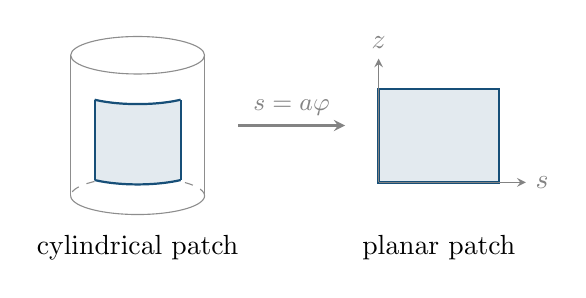
\begin{tikzpicture}[scale=0.85,>=stealth]
 \draw[ink!60] (-1,0)--(-1,2.1);
 \draw[ink!60] (1,0)--(1,2.1);
 \draw[ink!60,dashed] plot[domain=0:180,samples=35] ({cos(\x)},{0.28*sin(\x)});
 \draw[ink!60] plot[domain=180:360,samples=35] ({cos(\x)},{0.28*sin(\x)});
 \draw[ink!60] (0,2.1) ellipse (1 and 0.28);
 \fill[blue!12] plot[domain=230:310,samples=30] ({cos(\x)},{0.45+0.28*sin(\x)})
   -- plot[domain=310:230,samples=30] ({cos(\x)},{1.65+0.28*sin(\x)}) -- cycle;
 \draw[blue,thick] plot[domain=230:310,samples=30] ({cos(\x)},{0.45+0.28*sin(\x)});
 \draw[blue,thick] plot[domain=230:310,samples=30] ({cos(\x)},{1.65+0.28*sin(\x)});
 \draw[blue,thick] ({cos(230)},{0.45+0.28*sin(230)})--({cos(230)},{1.65+0.28*sin(230)});
 \draw[blue,thick] ({cos(310)},{0.45+0.28*sin(310)})--({cos(310)},{1.65+0.28*sin(310)});
 \node[below] at (0,-0.45) {cylindrical patch};
 \draw[->,thick,ink!65] (1.5,1.05)--(3.1,1.05)
   node[midway,above,font=\small] {\(s=a\varphi\)};
 \filldraw[fill=blue!12,draw=blue,thick] (3.6,0.2) rectangle (5.4,1.6);
 \draw[->,ink!65] (3.6,0.2)--(5.8,0.2) node[right] {\(s\)};
 \draw[->,ink!65] (3.6,0.2)--(3.6,2.05) node[above] {\(z\)};
 \node[below] at (4.5,-0.45) {planar patch};
\end{tikzpicture}
\end{center}

\subsection{Sectional curvature and the sphere}

Curvature can be assigned to a tangent two-plane rather than averaged
over all directions. Let \(u,v\in T_pM\) span a plane on which the
metric is nondegenerate. Thus
\(g(u,u)g(v,v)-g(u,v)^2\neq0\). Its \emph{sectional curvature} is
\begin{equation}
 K(u,v)=
 \frac{g\bigl(R(u,v)v,u\bigr)}
      {g(u,u)g(v,v)-g(u,v)^2}.
 \label{gr2:sectional-curvature}
\end{equation}
Both numerator and denominator acquire the same squared determinant
under a change of basis of the plane, so the quotient depends only
on the plane. For a Riemannian metric, every two-plane satisfies the
nondegeneracy condition. In two dimensions there is only one tangent
two-plane at each point. Its sectional curvature is the
\emph{Gaussian curvature}, and \eqref{gr2:two-dimensional-curvature}
gives \(R=2K\).

For the sphere of radius \(a\),
\[
 g=a^2\,\dd\vartheta^2+a^2\sin^2\vartheta\,\dd\varphi^2.
\]
The previously calculated component
\(R^\vartheta{}_{\varphi\vartheta\varphi}=\sin^2\vartheta\)
becomes
\[
 R_{\vartheta\varphi\vartheta\varphi}
 =a^2\sin^2\vartheta.
\]
Taking \(u=\partial_\vartheta\) and \(v=\partial_\varphi\) away
from the coordinate poles therefore yields
\begin{equation}
 K=\frac{a^2\sin^2\vartheta}{a^4\sin^2\vartheta}
   =\frac1{a^2},
 \qquad R=\frac2{a^2}.
 \label{gr2:sphere-sectional-curvature}
\end{equation}
These are scalar quantities and extend smoothly over the poles.
The Ricci contraction can also be evaluated directly. Reversing
both antisymmetric index pairs gives
\(R_{\varphi\vartheta\varphi\vartheta}
=R_{\vartheta\varphi\vartheta\varphi}\), so
\[
 R_{\vartheta\vartheta}
 =g^{\varphi\varphi}R_{\varphi\vartheta\varphi\vartheta}
 =\frac{a^2\sin^2\vartheta}{a^2\sin^2\vartheta}=1.
\]
The corresponding contraction gives
\(R_{\varphi\varphi}=\sin^2\vartheta\), and the mixed components
vanish. Hence \(\operatorname{Ric}=a^{-2}g\). Taking its trace
recovers the scalar curvature,
\[
 R=\frac{1}{a^2}\,1
  +\frac{1}{a^2\sin^2\vartheta}\,\sin^2\vartheta
  =\frac{2}{a^2}.
\]

If every nondegenerate tangent two-plane has the same sectional
curvature \(K\), the curvature tensor takes the form
\[
 R_{ijkl}=K(g_{ik}g_{jl}-g_{il}g_{jk}),
 \qquad R_{ij}=(n-1)Kg_{ij},
 \qquad R=n(n-1)K.
\]
The sphere illustrates this special case. Its scalar curvature
determines the radius because its geometry is already known to be
spherical. On a general manifold, sectional curvatures can differ
between planes. A single scalar cannot record those differences,
and \(R=0\) does not generally imply flatness. Scalar curvature has
dimensions of inverse length squared, but is not a universal local
curvature radius.

For a Riemannian metric this loss of information can be seen directly.
Choose an orthonormal basis \(e_1,\ldots,e_n\) at a point. The
denominator of \eqref{gr2:sectional-curvature} is then one for
each pair of distinct basis vectors, so
\[
 R=\sum_{i,j}g\bigl(R(e_i,e_j)e_j,e_i\bigr)
  =2\sum_{i<j}K(e_i,e_j).
\]
The zero terms with \(i=j\) drop out, and each remaining plane
appears twice in the first sum. Scalar curvature therefore sums
the sectional curvatures of the basis planes. Positive and
negative contributions can cancel, and different distributions
can produce the same sum. The sum is independent of the chosen
orthonormal basis even though the individual planes change.

\begin{studentwork}[2.7cm]{curvature under a constant rescaling}
Let \(\widetilde g=b^2g\) with constant \(b>0\). Determine how
\(\Gamma^i{}_{jk}\), \(R^i{}_{jkl}\), \(R_{ij}\), and the scalar
curvature change. Check the result for a sphere.
\end{studentwork}

\section{Orthonormal frames and tetrads}
\label{gr2:sec:frames}
\slidesref{15--16}

The coordinate calculations express geometry in terms of the functions
\(g_{\mu\nu}\) and \(\Gamma^\rho{}_{\mu\nu}\). An orthonormal frame gives
another description of the same geometry. Its metric components are
constant, while the variation of the frame is carried by its connection
coefficients. This is the local Lorentz-frame construction of GR1,
now developed into a method for calculating curvature.

Work on an open set \(U\) of a four-dimensional Lorentzian manifold.
Choose smooth vector fields \(e_a\), with \(a=0,1,2,3\), satisfying
\(g(e_a,e_b)=\eta_{ab}\), where
\(\eta=\operatorname{diag}(1,-1,-1,-1)\). Write the frame and its dual
coframe as
\begin{equation}
 e_a=e_a{}^\mu\partial_\mu,
 \qquad
 \varepsilon^a=\varepsilon^a{}_\mu\,\dd x^\mu,
 \qquad
 \varepsilon^a(e_b)=\delta^a{}_b.
 \label{gr2:eq:tetrad-frame}
\end{equation}
The coefficient matrices are inverse to one another. Consequently,
\begin{equation}
 \varepsilon^a{}_\mu e_b{}^\mu=\delta^a{}_b,
 \qquad
 e_a{}^\mu\varepsilon^a{}_\nu=\delta^\mu{}_\nu.
 \label{gr2:eq:tetrad-inverses}
\end{equation}
The frame is called a \emph{tetrad} or \emph{vierbein}. These terms
are also used for its coefficient matrix or the inverse coframe matrix.
Here the notation always distinguishes the two matrices.

The metric and its inverse have the representations
\begin{align}
 g&=\eta_{ab}\,\varepsilon^a\otimes\varepsilon^b,
 &g_{\mu\nu}&=\eta_{ab}\varepsilon^a{}_\mu\varepsilon^b{}_\nu,
 \label{gr2:eq:tetrad-metric}\\
 g^{\mu\nu}&=\eta^{ab}e_a{}^\mu e_b{}^\nu.
 \label{gr2:eq:tetrad-inverse-metric}
\end{align}
Greek indices refer to the coordinate basis and Latin indices to the
orthonormal frame. The metrics \(g_{\mu\nu}\) and \(\eta_{ab}\) raise
and lower indices of their respective kinds. The tetrad converts
between the two kinds. For a vector \(V\) and a covector \(A\),
\begin{equation}
 V^a=\varepsilon^a{}_\mu V^\mu,
 \qquad
 V^\mu=e_a{}^\mu V^a,
 \qquad
 A_a=e_a{}^\mu A_\mu.
 \label{gr2:eq:tetrad-conversion}
\end{equation}
For a mixed tensor, the same rule applies to each index separately,
\[
 Q^a{}_b=\varepsilon^a{}_\mu e_b{}^\nu Q^\mu{}_\nu.
\]
Thus a tetrad changes the representation of a tensor without changing
the tensor itself.

The distinction between index conversion and index lowering is useful
here. Lowering \(V^\mu\) produces the components of the metric-dual
covector. Multiplying by \(\varepsilon^a{}_\mu\) instead produces the
components of the original vector in another basis. Accordingly,
\(e_a{}^\mu\) and \(\varepsilon^a{}_\mu\) are inverse matrices, not
arrays obtained from one another merely by changing the placement of
an index. The metric relates them through
\[
 \varepsilon^a{}_\mu=\eta^{ab}g_{\mu\nu}e_b{}^\nu.
\]
This follows by taking the scalar product of \(e_b\) with
\(\partial_\mu=\varepsilon^c{}_\mu e_c\).

An orthonormal frame need not be a coordinate frame. Its vectors may
have nonzero Lie brackets, and its coframe forms need not be exact.
For instance, the orthonormal coframe on the sphere in GR1 satisfies
\(\dd\varepsilon^2\neq0\). Constant metric components in such a frame
therefore do not imply zero curvature. All constructions here are
local. A single smooth orthonormal frame on the entire manifold is
not assumed.

\begin{studentwork}[1.7cm]{constant metric components}
Why can \(g(e_a,e_b)=\eta_{ab}\) hold throughout a neighborhood
with nonzero curvature? Explain the difference from constant metric
components in a coordinate basis.
\end{studentwork}

\subsection{Coordinate changes and local Lorentz transformations}

Under a coordinate change \(x^\mu\mapsto x'{}^\nu\), keep the
geometric frame fixed. Its coefficients transform as
\[
 e_a{}^{\nu'}=\frac{\partial x'{}^\nu}{\partial x^\mu}e_a{}^\mu,
 \qquad
 \varepsilon^a{}_{\nu'}=
 \frac{\partial x^\mu}{\partial x'{}^\nu}\varepsilon^a{}_\mu.
\]
These are the usual transformations of a vector and a covector.
Alternatively, keep the coordinates fixed and choose a different
orthonormal frame. Following the component convention of SR1 and GR1,
write
\begin{equation}
 e'_a=e_b(\Lambda^{-1})^b{}_a,
 \qquad
 \Lambda^{\mathsf T}\eta\Lambda=\eta.
 \label{gr2:eq:llt-frame}
\end{equation}
Here \(\Lambda:U\to O(1,3)\) is a smooth matrix-valued function.
Duality and the equality \(V=V^a e_a=V'^a e'_a\) then give
\begin{equation}
 \varepsilon'^a=\Lambda^a{}_b\varepsilon^b,
 \qquad
 V'^a=\Lambda^a{}_b V^b,
 \qquad
 A'_a=(\Lambda^{-1})^b{}_a A_b.
 \label{gr2:eq:llt-components}
\end{equation}
The word \emph{local} allows the Lorentz matrix to vary with position.
Equation~\eqref{gr2:eq:llt-frame} preserves
\eqref{gr2:eq:tetrad-metric}, so both frames describe the same metric.

Coordinate changes act on the Greek indices, while frame changes act
on the Latin indices. Both freedoms remain available. A tetrad has
sixteen component functions, with six local Lorentz freedoms. This
leaves the ten independent functions of a symmetric metric. The
tetrad description reorganizes the metric information together with
a choice of frame.

For an observer with four-velocity \(u\) normalized by
\(g(u,u)=c^2\), choose \(e_0=u/c\) at that point.
The three spacelike frame vectors then provide
orthogonal spatial directions for that observer. This interpretation
concerns a basis of one tangent space. Extending the basis smoothly
over a neighborhood provides a family of local frames, and does not
by itself provide coordinates on that neighborhood.

\begin{studentwork}[2.5cm]{converting tensor components}
Express \(Q^\mu{}_\nu\) in terms of \(Q^a{}_b\).
Show that \(Q^a{}_a=Q^\mu{}_\mu\).
\end{studentwork}

\section{The connection in an orthonormal frame}
\label{gr2:sec:spin-connection}
\slideref{17}

Let \(\nabla\) be an affine connection. Define its coefficients in the
orthonormal frame by
\begin{equation}
 \nabla_{\partial_\mu}e_b=\omega_\mu{}^a{}_b e_a,
 \qquad
 \omega^a{}_b=\omega_\mu{}^a{}_b\,\dd x^\mu.
 \label{gr2:eq:spin-definition}
\end{equation}
The matrix \(\omega=(\omega^a{}_b)\) is the connection one-form in this
frame. For a metric-compatible connection it is commonly called the
\emph{spin connection}. Here its action is needed only on vectors and tensors.

Differentiating \(V=V^b e_b\) gives
\begin{equation}
 (\nabla_\mu V)^a
 =\partial_\mu V^a+\omega_\mu{}^a{}_bV^b.
 \label{gr2:eq:frame-vector-derivative}
\end{equation}
Preservation of the pairing \(A_aV^a\) determines the sign for a lower
frame index. Thus
\begin{align}
 (\nabla_\mu A)_a
 &=\partial_\mu A_a-\omega_\mu{}^b{}_aA_b,\\
 (\nabla_\mu Q)^a{}_b
 &=\partial_\mu Q^a{}_b
   +\omega_\mu{}^a{}_cQ^c{}_b
   -\omega_\mu{}^c{}_bQ^a{}_c.
 \label{gr2:eq:frame-tensor-derivative}
\end{align}
These are the tensor differentiation rules already obtained for
coordinate indices, now applied to the moving orthonormal frame.

\subsection{Relating the two connection matrices}

The coefficients \(\Gamma^\rho{}_{\mu\nu}\) and
\(\omega_\mu{}^a{}_b\) describe the same derivative in different
frames. To find their relation, substitute
\(V^a=\varepsilon^a{}_\nu V^\nu\) into
\eqref{gr2:eq:frame-vector-derivative}. Expressing the answer in the
coordinate basis gives
\begin{align*}
 e_a{}^\rho(\nabla_\mu V)^a
 &=e_a{}^\rho\left[
 \partial_\mu(\varepsilon^a{}_\nu V^\nu)
 +\omega_\mu{}^a{}_b\varepsilon^b{}_\nu V^\nu\right]\\
 &=e_a{}^\rho\varepsilon^a{}_\nu\,\partial_\mu V^\nu
 +e_a{}^\rho(\partial_\mu\varepsilon^a{}_\nu)V^\nu
 +e_a{}^\rho\omega_\mu{}^a{}_b\varepsilon^b{}_\nu V^\nu\\
 &=\partial_\mu V^\rho+
 e_a{}^\rho\left(
 \partial_\mu\varepsilon^a{}_\nu
 +\omega_\mu{}^a{}_b\varepsilon^b{}_\nu\right)V^\nu.
\end{align*}
The first term reduces to \(\partial_\mu V^\rho\) because
\(e_a{}^\rho\varepsilon^a{}_\nu=\delta^\rho{}_\nu\).
Since the result equals \(\partial_\mu V^\rho+
\Gamma^\rho{}_{\mu\nu}V^\nu\) for every vector field,
\begin{equation}
 \Gamma^\rho{}_{\mu\nu}
 =e_a{}^\rho\left(
 \partial_\mu\varepsilon^a{}_\nu
 +\omega_\mu{}^a{}_b\varepsilon^b{}_\nu\right).
 \label{gr2:eq:gamma-from-spin}
\end{equation}
Equivalently,
\begin{equation}
 \omega_\mu{}^a{}_b
 =\varepsilon^a{}_\rho\left(
 \partial_\mu e_b{}^\rho+
 \Gamma^\rho{}_{\mu\nu}e_b{}^\nu\right).
 \label{gr2:eq:spin-from-gamma}
\end{equation}
The derivative of the frame is essential. A connection cannot be
converted by multiplying tetrad matrices alone.

Multiplying \eqref{gr2:eq:gamma-from-spin} by
\(\varepsilon^a{}_\rho\) yields the \emph{tetrad postulate},
\begin{equation}
 \mathcal D_\mu\varepsilon^a{}_\nu
 :=\partial_\mu\varepsilon^a{}_\nu
   -\Gamma^\rho{}_{\mu\nu}\varepsilon^a{}_\rho
   +\omega_\mu{}^a{}_b\varepsilon^b{}_\nu=0.
 \label{gr2:eq:tetrad-postulate}
\end{equation}
The symbol \(\mathcal D_\mu\) indicates that both the coordinate
index and the frame index are differentiated. This identity states
that conversion of components commutes with covariant
differentiation. Once \(\omega\) is defined from \(\nabla\) and the
frame, it is an identity, not an additional condition on the geometry.
In particular, it holds for connections with torsion.

\subsection{Transformation of the spin connection}
\slideref{18}

For a fixed orthonormal frame, \(\omega^a{}_b\) is a one-form under
coordinate changes. Its frame transformation contains an additional
term because \(\Lambda\) can depend on position. Write the component
column derivative as
\[
 DV=\dd V+\omega V.
\]
It must satisfy \(D'V'=\Lambda DV\). Using \(V'=\Lambda V\),
\[
 D'V'=\dd(\Lambda V)+\omega'\Lambda V
 =\Lambda\dd V+(\dd\Lambda+\omega'\Lambda)V.
\]
Comparison for arbitrary \(V\) determines
\begin{equation}
 \boxed{\omega'=\Lambda\omega\Lambda^{-1}
                   -\dd\Lambda\,\Lambda^{-1}.}
 \label{gr2:eq:spin-transformation}
\end{equation}
The last term compensates for differentiating the varying Lorentz
matrix. It vanishes for a constant frame transformation. This is the
frame version of the inhomogeneous coordinate transformation law
for \(\Gamma^\rho{}_{\mu\nu}\).

\begin{studentwork}[2.5cm]{the inverse tetrad identity}
Differentiate \(\varepsilon^a{}_\rho e_b{}^\rho=\delta^a{}_b\)
and use the tetrad postulate to derive
\eqref{gr2:eq:spin-from-gamma}.
\end{studentwork}

\section{Covariant exterior differentiation}
\label{gr2:sec:covariant-exterior}
\slidesref{18--19}

Differential forms keep antisymmetric coordinate indices together.
They are therefore particularly useful for torsion and curvature,
whose final two indices are antisymmetric. To differentiate forms
that also carry frame indices, combine the exterior derivative with
the connection acting on those indices.

A tangent-vector-valued \(k\)-form can be written
\(\alpha=e_a\otimes\alpha^a\), where each
\(\alpha^a\in\Omega^k(U)\) is an ordinary differential form.
Its components transform as \(\alpha'^a=\Lambda^a{}_b\alpha^b\).
Define the \emph{covariant exterior derivative} by
\begin{equation}
 (D\alpha)^a=\dd\alpha^a+\omega^a{}_b\wedge\alpha^b.
 \label{gr2:eq:covariant-exterior-vector}
\end{equation}
The result is a vector-valued \((k+1)\)-form. Substitution of
\eqref{gr2:eq:spin-transformation} shows that
\((D\alpha)'{}^a=\Lambda^a{}_b(D\alpha)^b\). For a covector-valued
form \(\beta_a\), the corresponding rule is
\[
 (D\beta)_a=\dd\beta_a-\omega^b{}_a\wedge\beta_b.
\]
For \(k=0\), equation~\eqref{gr2:eq:covariant-exterior-vector}
recovers the vector derivative above.

\begin{remarkbox}[Derivative notation]
\(\dd\) acts on ordinary scalar-valued differential forms. It increases
form degree by one and requires no connection.

\(D\) acts on forms that also carry vector or tensor indices. It
increases form degree by one and adds connection terms for those
indices, as in \eqref{gr2:eq:covariant-exterior-vector}.

\(\mathcal D_\mu\) is the full component covariant derivative.
It includes a connection term for every tensor index, using
\(\Gamma\) for coordinate indices and \(\omega\) for frame indices.
The new differentiation index \(\mu\) is retained rather than
antisymmetrized with the form indices.
\end{remarkbox}

For a vector-valued one-form \(\alpha^a=\alpha^a{}_\nu\dd x^\nu\),
the component convention is
\begin{align}
 (D\alpha)^a&=\frac12(D\alpha)^a{}_{\mu\nu}
                     \dd x^\mu\wedge\dd x^\nu,\\
 (D\alpha)^a{}_{\mu\nu}
 &=\partial_\mu\alpha^a{}_\nu-\partial_\nu\alpha^a{}_\mu
 +\omega_\mu{}^a{}_b\alpha^b{}_\nu
 -\omega_\nu{}^a{}_b\alpha^b{}_\mu.
 \label{gr2:eq:covariant-exterior-components}
\end{align}
The factor \(1/2\) counts each antisymmetric pair once. The exterior
derivative already handles the form indices, so the displayed
definition adds connection terms only for the frame index.

For comparison, the full derivative of the component array is
\[
 \mathcal D_\mu\alpha^a{}_\nu
 =\partial_\mu\alpha^a{}_\nu
 +\omega_\mu{}^a{}_b\alpha^b{}_\nu
 -\Gamma^\rho{}_{\mu\nu}\alpha^a{}_\rho.
\]
Subtracting the expression with \(\mu\) and \(\nu\) exchanged gives
\[
 \mathcal D_\mu\alpha^a{}_\nu-\mathcal D_\nu\alpha^a{}_\mu
 =(D\alpha)^a{}_{\mu\nu}
 -\bigl(\Gamma^\rho{}_{\mu\nu}-\Gamma^\rho{}_{\nu\mu}\bigr)
   \alpha^a{}_\rho.
\]
The expression in parentheses is \(T^\rho{}_{\mu\nu}\) in a coordinate
basis.
Moving this term to the other side gives
\[
 (D\alpha)^a{}_{\mu\nu}
 =\mathcal D_\mu\alpha^a{}_\nu
  -\mathcal D_\nu\alpha^a{}_\mu
  +T^\rho{}_{\mu\nu}\alpha^a{}_\rho.
\]
For the Levi--Civita connection the torsion term vanishes, and
covariant exterior differentiation is antisymmetrized covariant
differentiation. The definition using \(\dd\) and \(\omega\) remains
valid for any connection. This distinction is especially useful when
the one-form being differentiated is the coframe itself.

Matrix-valued forms require both matrix multiplication and the wedge
product. Our notation means
\[
 (A\wedge B)^a{}_b=A^a{}_c\wedge B^c{}_b.
\]
Their factors generally cannot be exchanged using a sign alone,
because the matrix coefficients need not commute. For an
endomorphism-valued \(k\)-form \(A=(A^a{}_b)\), covariant exterior
differentiation takes the form
\begin{equation}
 DA=\dd A+\omega\wedge A-(-1)^kA\wedge\omega.
 \label{gr2:eq:covariant-exterior-matrix}
\end{equation}
The final term differentiates the lower frame index. Its degree sign
appears when the connection one-form is moved past the \(k\)-form.
In particular, for a matrix of functions,
\(DA=\dd A+\omega A-A\omega\).

\subsection{Torsion and the first structure equation}

The collection \(\varepsilon^a\) represents the tangent-vector-valued
one-form given by the identity map \(X\mapsto X\), since
\(X=\varepsilon^a(X)e_a\). Its covariant exterior derivative measures
torsion. To see this, evaluate it on vector fields \(X,Y\),
\begin{align*}
 (D\varepsilon)^a(X,Y)
 &=X\bigl(\varepsilon^a(Y)\bigr)
   -Y\bigl(\varepsilon^a(X)\bigr)-\varepsilon^a([X,Y])\\
 &\quad+\omega^a{}_b(X)\varepsilon^b(Y)
       -\omega^a{}_b(Y)\varepsilon^b(X)\\
 &=\varepsilon^a\bigl(\nabla_XY-\nabla_YX-[X,Y]\bigr).
\end{align*}
Thus the torsion two-forms satisfy the first Cartan structure equation,
\begin{equation}
 \boxed{T^a=\dd\varepsilon^a+\omega^a{}_b\wedge\varepsilon^b,}
 \qquad
 T^a=\frac12\varepsilon^a{}_\rho T^\rho{}_{\mu\nu}
                  \dd x^\mu\wedge\dd x^\nu.
 \label{gr2:eq:cartan-torsion}
\end{equation}
For a torsion-free connection this becomes an equation for the
connection one-forms in terms of the chosen coframe.

This equation also incorporates the noncommutativity of the frame.
Write \([e_b,e_c]=C^a{}_{bc}e_a\). The coframe identity from GR1 is
\(\dd\varepsilon^a(e_b,e_c)=-C^a{}_{bc}\), so
\[
 T^a(e_b,e_c)
 =\omega^a{}_c(e_b)-\omega^a{}_b(e_c)-C^a{}_{bc}.
\]
Thus zero torsion does not require the frame connection coefficients
to be symmetric in the direction and vector indices. Their
antisymmetric part compensates for the Lie bracket of the frame
vectors. The familiar symmetry of the lower Christoffel indices is
the coordinate-frame case, where all these brackets vanish. In the
structure equation this distinction is contained in
\(\dd\varepsilon^a\), so no separate bracket correction needs to be
added during the calculation.

The operators \(D\) and \(\mathcal D_\mu\) in the tetrad postulate
serve different purposes. The latter differentiates every component
index. Antisymmetrizing the tetrad postulate gives
\[
 (D\varepsilon)^a{}_{\mu\nu}
 =\varepsilon^a{}_\rho
   \bigl(\Gamma^\rho{}_{\mu\nu}-\Gamma^\rho{}_{\nu\mu}\bigr),
\]
which can be nonzero even though
\(\mathcal D_\mu\varepsilon^a{}_\nu=0\).

\subsection{Curvature and the second structure equation}

Apply \(D\) twice to a vector-component column \(V\). The ordinary
exterior derivative satisfies \(\dd^2=0\), but the connection adds
terms,
\begin{align*}
 D^2V
 &=\dd(\dd V+\omega V)+\omega\wedge(\dd V+\omega V)\\
 &=(\dd\omega)V-\omega\wedge\dd V
            +\omega\wedge\dd V+(\omega\wedge\omega)V\\
 &=(\dd\omega+\omega\wedge\omega)V.
\end{align*}
This defines the curvature two-form and gives the second Cartan
structure equation,
\begin{equation}
 \boxed{\mathcal R^a{}_b
       =\dd\omega^a{}_b+\omega^a{}_c\wedge\omega^c{}_b,}
 \qquad D^2V^a=\mathcal R^a{}_bV^b.
 \label{gr2:eq:cartan-curvature}
\end{equation}
Evaluation on two vector fields gives the curvature operator,
\[
 \mathcal R^a{}_b(X,Y)V^b
 =\varepsilon^a\bigl(R(X,Y)V\bigr).
\]
The coordinate and frame descriptions are therefore related by
\begin{equation}
 \mathcal R^a{}_b
 =\frac12\varepsilon^a{}_\rho e_b{}^\sigma
 R^\rho{}_{\sigma\mu\nu}\,\dd x^\mu\wedge\dd x^\nu
 =\frac12R^a{}_{bcd}\,\varepsilon^c\wedge\varepsilon^d.
 \label{gr2:eq:curvature-form-components}
\end{equation}
The two-form notation packages the antisymmetric direction indices.
It does not change the curvature convention or add a new curvature
tensor. Under a local Lorentz change,
\[
 T'^a=\Lambda^a{}_bT^b,
 \qquad
 \mathcal R'=\Lambda\mathcal R\Lambda^{-1}.
\]
The inhomogeneous terms in the connection transformation cancel from
these tensorial quantities.

The same calculation also applies to a vector-valued form of any
degree. The product rule gives
\(\dd(\omega\wedge\alpha)=\dd\omega\wedge\alpha
-\omega\wedge\dd\alpha\), so the terms containing
\(\dd\alpha\) cancel and
\[
 D^2\alpha^a=\mathcal R^a{}_b\wedge\alpha^b.
\]
Thus \(D\) generally fails to square to zero. Its failure is measured
precisely by curvature acting on the vector-valued part of the form.
Ordinary scalar-valued forms have no frame index, and their ordinary
exterior derivative still satisfies \(\dd^2=0\).

\begin{studentwork}[2.5cm]{curvature acting on covectors}
Starting from \((DA)_a=\dd A_a-\omega^b{}_aA_b\), show that
\(D^2A_a=-\mathcal R^b{}_aA_b\).
\end{studentwork}

\subsection{The Bianchi identities}

Both Bianchi identities follow from the structure equations and the
graded product rule. First, differentiate the torsion equation,
\begin{align*}
 DT^a
 &=\dd\bigl(\dd\varepsilon^a+
             \omega^a{}_b\wedge\varepsilon^b\bigr)
   +\omega^a{}_b\wedge
       \bigl(\dd\varepsilon^b+\omega^b{}_c\wedge\varepsilon^c\bigr)\\
 &=(\dd\omega^a{}_b)\wedge\varepsilon^b
   -\omega^a{}_b\wedge\dd\varepsilon^b
   +\omega^a{}_b\wedge\dd\varepsilon^b
   +\omega^a{}_b\wedge\omega^b{}_c\wedge\varepsilon^c.
\end{align*}
The middle terms cancel. Relabeling the summed frame indices gives
\begin{equation}
 \boxed{DT^a=\mathcal R^a{}_b\wedge\varepsilon^b.}
 \label{gr2:eq:first-bianchi-forms}
\end{equation}
When \(T=0\), the right-hand side vanishes. Evaluation on three
vector fields yields
\(R(X,Y)Z+R(Y,Z)X+R(Z,X)Y=0\), the algebraic first Bianchi identity.
Equation~\eqref{gr2:eq:first-bianchi-forms} also states its form for
a connection with torsion.

For the curvature matrix, equation~\eqref{gr2:eq:covariant-exterior-matrix}
with degree two gives
\[
 D\mathcal R=\dd\mathcal R+
              \omega\wedge\mathcal R-\mathcal R\wedge\omega.
\]
The structure equation implies
\begin{align*}
 \dd\mathcal R&=\dd\omega\wedge\omega
                        -\omega\wedge\dd\omega,\\
 \omega\wedge\mathcal R-\mathcal R\wedge\omega
 &=\omega\wedge\dd\omega-\dd\omega\wedge\omega.
\end{align*}
The cubic terms cancel by associativity of matrix multiplication and
the wedge product. Hence the differential Bianchi identity is
\begin{equation}
 \boxed{D\mathcal R=0.}
 \label{gr2:eq:second-bianchi-forms}
\end{equation}
For the Levi--Civita connection, its coordinate expression is
\[
 \nabla_\lambda R^\rho{}_{\sigma\mu\nu}
 +\nabla_\mu R^\rho{}_{\sigma\nu\lambda}
 +\nabla_\nu R^\rho{}_{\sigma\lambda\mu}=0.
\]
Thus the compact form equations reproduce the curvature identities
used earlier, while making their origin in the connection explicit.

\subsection{Metric compatibility in the orthonormal frame}

The frame metric has constant entries. Metric compatibility therefore
reduces to
\[
 0=(\nabla_\mu\eta)_{ab}
 =-\omega_\mu{}^c{}_a\eta_{cb}
  -\omega_\mu{}^c{}_b\eta_{ac}.
\]
Define \(\omega_{ab}=\eta_{ac}\omega^c{}_b\). Then
\begin{equation}
 \omega_{ab}=-\omega_{ba}.
 \label{gr2:eq:spin-antisymmetry}
\end{equation}
The antisymmetry applies after lowering the first frame index.
For a positive-definite orthonormal frame, \(\eta_{ab}\) is replaced
by \(\delta_{ab}\), so the mixed-index matrix is antisymmetric as well.
Together with \(T^a=0\), equation~\eqref{gr2:eq:spin-antisymmetry}
determines the Levi--Civita connection in a chosen orthonormal frame.
The following calculations use these two conditions directly.

For Lorentzian signature the location of the indices matters even
for this simple condition. For a spatial index \(i\),
\(\omega_{0i}=\omega^0{}_i\) and
\(\omega_{i0}=-\omega^i{}_0\), so antisymmetry implies
\(\omega^0{}_i=\omega^i{}_0\). The mixed matrix is therefore not
an ordinary antisymmetric real matrix. It obeys
\(\omega^{\mathsf T}\eta+\eta\omega=0\), which is the infinitesimal
form of the Lorentz condition.

In practice, one first computes \(\dd\varepsilon^a\), then solves
\(\dd\varepsilon^a+\omega^a{}_b\wedge\varepsilon^b=0\)
together with metric compatibility. These equations determine the
connection uniquely by the Levi--Civita theorem. Finally, the second
structure equation gives the curvature. This method avoids
calculating all coordinate Christoffel symbols when the metric has
a simple orthonormal coframe.

\subsection{Flat space and the sphere revisited}

\begin{examplebox}{Euclidean space in a spherical coframe}{gr2:flat-cartan}
On a spherical coordinate patch with \(r>0\) and
\(0<\vartheta<\pi\), take
\[
 \varepsilon^1=\dd r,\qquad
 \varepsilon^2=r\,\dd\vartheta,\qquad
 \varepsilon^3=r\sin\vartheta\,\dd\varphi.
\]
The Euclidean metric is \(g=\delta_{ab}\varepsilon^a\otimes\varepsilon^b\).
The exterior derivatives are
\begin{align*}
 \dd\varepsilon^1&=0,\\
 \dd\varepsilon^2&=\frac1r\varepsilon^1\wedge\varepsilon^2,\\
 \dd\varepsilon^3&=(\sin\vartheta\,\dd r
                   +r\cos\vartheta\,\dd\vartheta)\wedge\dd\varphi\\
 &=\frac1r\varepsilon^1\wedge\varepsilon^3
             +\frac{\cot\vartheta}{r}\varepsilon^2\wedge\varepsilon^3.
\end{align*}
These derivatives suggest trying
\(\omega^1{}_2=A\varepsilon^2\),
\(\omega^1{}_3=B\varepsilon^3\), and
\(\omega^2{}_3=C\varepsilon^3\), with scalar coefficient functions
\(A,B,C\), together with antisymmetry. It is enough to find a solution
of all three torsion equations, since metric compatibility and zero
torsion determine the connection uniquely.
The first torsion equation is then automatic. The second becomes
\[
 0=\dd\varepsilon^2+\omega^2{}_1\wedge\varepsilon^1
                      +\omega^2{}_3\wedge\varepsilon^3
   =\left(\frac1r+A\right)\varepsilon^1\wedge\varepsilon^2,
\]
so \(A=-1/r\). For the third equation, use
\(\omega^3{}_1=-B\varepsilon^3\) and
\(\omega^3{}_2=-C\varepsilon^3\). Then
\begin{align*}
 0=T^3
 &=\dd\varepsilon^3+\omega^3{}_1\wedge\varepsilon^1
                       +\omega^3{}_2\wedge\varepsilon^2\\
 &=\frac1r\varepsilon^1\wedge\varepsilon^3
   +\frac{\cot\vartheta}{r}\varepsilon^2\wedge\varepsilon^3
   -B\varepsilon^3\wedge\varepsilon^1
   -C\varepsilon^3\wedge\varepsilon^2\\
 &=\left(\frac1r+B\right)\varepsilon^1\wedge\varepsilon^3
   +\left(\frac{\cot\vartheta}{r}+C\right)
      \varepsilon^2\wedge\varepsilon^3.
\end{align*}
The two basis two-forms are linearly independent. Their coefficients
must vanish separately, so \(B=-1/r\) and
\(C=-\cot\vartheta/r\). Substituting the coframe gives
\[
 \omega^1{}_2=-\dd\vartheta,\qquad
 \omega^1{}_3=-\sin\vartheta\,\dd\varphi,\qquad
 \omega^2{}_3=-\cos\vartheta\,\dd\varphi,
\]
with \(\omega^b{}_a=-\omega^a{}_b\) and zero diagonal entries.
For example, the angular curvature two-form is
\begin{align*}
 \mathcal R^2{}_3
 &=\dd\omega^2{}_3+\omega^2{}_1\wedge\omega^1{}_3\\
 &=\sin\vartheta\,\dd\vartheta\wedge\dd\varphi
   +(\dd\vartheta)\wedge(-\sin\vartheta\,\dd\varphi)=0.
\end{align*}
The other curvature forms also vanish. The nonzero connection
describes the variation of this frame in flat Euclidean space.
\end{examplebox}

\begin{studentwork}[2.5cm]{flatness in the spherical frame}
For the connection above, calculate
\(\mathcal R^1{}_2\) and \(\mathcal R^1{}_3\).
\end{studentwork}

\begin{examplebox}{Curvature of the sphere from its coframe}{gr2:sphere-cartan}
For the sphere of radius \(a>0\), use
\[
 \varepsilon^1=a\,\dd\vartheta,\qquad
 \varepsilon^2=a\sin\vartheta\,\dd\varphi.
\]
Here
\[
 \dd\varepsilon^1=0,\qquad
 \dd\varepsilon^2=\frac{\cot\vartheta}{a}
                          \varepsilon^1\wedge\varepsilon^2.
\]
The torsion-free equations are
\[
 \omega^1{}_2\wedge\varepsilon^2=0,\qquad
 \dd\varepsilon^2+\omega^2{}_1\wedge\varepsilon^1=0.
\]
Writing \(\omega^1{}_2=A\varepsilon^1+B\varepsilon^2\), the first
equation reads \(A\varepsilon^1\wedge\varepsilon^2=0\), so \(A=0\).
Using \(\omega^2{}_1=-B\varepsilon^2\), the second becomes
\[
 0=\frac{\cot\vartheta}{a}\varepsilon^1\wedge\varepsilon^2
      -B\varepsilon^2\wedge\varepsilon^1
   =\left(\frac{\cot\vartheta}{a}+B\right)
      \varepsilon^1\wedge\varepsilon^2.
\]
Thus \(B=-\cot\vartheta/a\). Therefore
\[
 \omega^1{}_2=-\cos\vartheta\,\dd\varphi,
 \qquad
 \mathcal R^1{}_2=\dd\omega^1{}_2
 =\sin\vartheta\,\dd\vartheta\wedge\dd\varphi
 =\frac1{a^2}\varepsilon^1\wedge\varepsilon^2.
\]
There is no third frame direction and no quadratic connection term
in this curvature component. Reading its coefficient gives
\(R^1{}_{212}=1/a^2\), in agreement with the coordinate calculation.
Thus the Gaussian curvature is \(K=1/a^2\) and the scalar curvature
is \(R=2/a^2\).
\end{examplebox}

The angular part of the Euclidean spherical connection resembles
the sphere connection, but their curvature calculations include
different frame directions. In Euclidean space, the terms involving
the radial direction cancel the angular derivative term. On the
sphere, the connection acts only within its two-dimensional tangent
spaces, and its intrinsic curvature is nonzero.

\begin{studentwork}[2.5cm]{Ricci curvature in the sphere frame}
Use \(\mathcal R^1{}_2=a^{-2}\varepsilon^1\wedge\varepsilon^2\)
and curvature antisymmetry to find \(R_{11},R_{22},R_{12}\).
Contract them to obtain the scalar curvature.
\end{studentwork}

\section{Metric, connection, and curvature}
\slideref{20}

The metric determines scalar products and selects the Levi--Civita
connection. This connection defines parallel transport, and curvature
measures the leading change around a small loop. Nonzero connection
coefficients can reflect a varying basis in flat space. Nonzero
curvature is an intrinsic obstruction to a parallel frame throughout a
neighborhood.

Coordinate bases and orthonormal frames give equivalent descriptions.
The coframe records the metric, while the connection and curvature
can be represented as follows.
\[
 \begin{aligned}
 \nabla_{\partial_\mu}\partial_\nu
   &=\Gamma^\rho{}_{\mu\nu}\partial_\rho,
 &\nabla e_b&=e_a\otimes\omega^a{}_b,\\
 R(\partial_\mu,\partial_\nu)\partial_\sigma
   &=R^\rho{}_{\sigma\mu\nu}\partial_\rho,
 &\mathcal R^a{}_b
   &=\dd\omega^a{}_b+\omega^a{}_c\wedge\omega^c{}_b.
 \end{aligned}
\]
Here the tensor-valued one-form \(\nabla e_b\) sends \(X\)
to \(\nabla_Xe_b\).

In the frame description, \(T^a=0\) and
\(\omega_{ab}=-\omega_{ba}\) together determine the Levi--Civita
connection. Coordinate transformations remain available, and local
Lorentz transformations express the freedom to choose an orthonormal
frame at each event.

\end{document}